\documentclass[11pt,draft,phd]{osudiss-2}

% cli to extract pages from pdf
% qpdf input.pdf --pages . 1-10 -- output.pdf

\usepackage[english]{babel}
\usepackage{microtype}
\usepackage{environ}
\usepackage{amsmath}
\usepackage[numbers,sort&compress]{natbib}
\usepackage{doi}
\usepackage{graphicx}
\usepackage{rotating}
\usepackage{tabularx}
\usepackage{dcolumn}
\usepackage{booktabs}
\usepackage{scrextend} % for \footref
\usepackage{hyperref}
\usepackage[nameinlink,capitalize]{cleveref}
\usepackage{siunitx}
\usepackage{enumitem}
\usepackage{floatrow}
\usepackage{bm}
\usepackage{mathtools}

%\usepackage[acronym, section=chapter]{glossaries}
%\makeglossaries
%\include{acronyms}

\usepackage{lipsum}

% style stuff
\bibliographystyle{apsrev4-1-custom}
\addto{\captionsenglish}{\renewcommand{\bibname}{References}}
\hypersetup{hidelinks}

% custom commands
\DeclareMathOperator{\Tanh}{\mathbf{tanh}}
\DeclarePairedDelimiter\ceil{\lceil}{\rceil}
\DeclarePairedDelimiter\floor{\lfloor}{\rfloor}

% environment for figure re-use
% https://tex.stackexchange.com/a/225075
% \begin{reusefigure}[<float spec>]{<ref>}
%\newenvironment{reusefigure}[2][tbp]
%  {\addtocounter{figure}{-1}%
%   \renewcommand{\theHfigure}{dupe-fig}% If you're using hyperref
%   \renewcommand{\thefigure}{\ref{#2}}% Figure counter is \ref
%   \renewcommand{\addcontentsline}[3]{}% Avoid placing figure in LoF
%   \begin{figure}[#1]}
%  {\end{figure}}

% use dcolumn
\newcolumntype{d}{D{.}{.}{-1}}
\newcolumntype{e}{D{.}{.}{8}}
\newcolumntype{f}{D{.}{.}{13}}

% full references with names
\newcommand*{\fullref}[1]{\hyperref[{#1}]{\Cref*{#1} \nameref*{#1}}}

\title{Essential Reservoir Computing}
\author{Aaron Griffith}
\advisorname{Daniel J. Gauthier}
\degree{Doctor of Philosophy}
\member{Amy Connolly}
\member{Ciriyam Jayaprakash}
\member{Gregory Lafyatis}
\authordegrees{B.S.}
\graduationyear{2021}
\unit{Graduate Program in Physics}

\begin{document}

\frontmatter

\begin{abstract}
  % abstract: 500 words or less

  \emph{Reservoir computing} (RC) is a machine learning method
  especially well suited to solving physical problems, by using an
  internal dynamic system known as a 'reservoir'. Many systems are
  suitable for use as an internal reservoir. A common choice is an
  \emph{echo state network} (ESN), a network with recurrent
  connections that gives the RC a memory which it uses to efficiently
  solve many time-domain problems such as forecasting chaotic systems
  and hidden state inference. However, constructing an ESN involves a
  large number of poorly-understood meta-parameters, and the properties
  that an ESN must have to solve these tasks well are largely unknown.

  In this dissertation, I explore what parts of an RC are absolutely
  necessary. I build ESNs that perform well at system forecasting
  despite an extremely simple internal network structure, without any
  recurrent connections at all, breaking one of the most common rules
  of ESN design. These simple reservoirs indicate that the role of the
  reservoir in the RC is only to remember a finite number of
  time-delays of the RCs input, and while a complicated network can
  achieve this, in many cases a simple one achieves this as well.

  I then build upon a recent proof of the equivalence between a
  specific ESN construction and the nonlinear vector auto-regression
  (NVAR) method with my collaborators. The NVAR is an RC boiled down
  to its most essential components, taking the necessary time-delay
  taps directly rather than relying on an internal dynamic
  reservoir. I demonstrate these RCs-without-reservoirs on a variety
  of classical RC problems, showing that in many cases an NVAR will
  perform as well or better than an RC despite the simpler
  method. I then conclude with an example problem that highlights a
  remaining unsolved issue in the application of NVARs, and then look
  to a possible future where NVARs may supplant RCs.
\end{abstract}

\dedication{For my brother Nathan, and my parents Gregory and Mary Lea.}

\begin{acknowledgments}
  This work would not have been possible without the committed support
  of my advisor, Daniel~J.~Gauthier, or my insightful collaborators,
  including Wendson~A.~S.~Barbosa, Erik~Bollt, Daniel~Canaday, and Andrew~Pomerance.

  In addition, many discussions over the years have
  re-contextualized my understanding of reservoir computers. I would
  specifically like to thank Michelle~Girvan, Brian~Hunt, and Edward~Ott.
\end{acknowledgments}

\begin{vita}
  \dateitem{2009-2014}{B.S., Mathematics and Physics \\ The Ohio State University}
  \dateitem{2015-2016}{Graduate Teaching Associate \\ Department of Physics \\ The Ohio State University}
  \dateitem{2016-2021}{Graduate Research Associate \\ Department of Physics \\ The Ohio State University}

  \begin{publist}
    \pubitem{D.~Canaday, A.~Griffith, and D.~J.~Gauthier, ``Rapid time series prediction with a hardware-based reservoir computer,'' \href{https://doi.org/10.1063/1.5048199}{Chaos: An Interdisciplinary Journal of Nonlinear Science \textbf{28}, 123119 (2018)}.}
    \pubitem{A.~Griffith, A.~Pomerance, and D.~J.~Gauthier, ``Forecasting chaotic systems with very low connectivity reservoir computers,'' \href{https://doi.org/10.1063/1.5120710}{Chaos: An Interdisciplinary Journal of Nonlinear Science \textbf{29}, 123108 (2019)}.}
    %\pubitem{W.~A.~S.~Barbosa, A.~Griffith, G.~E.~Rowlands, L.~C.~G.~Govia, G.~J.~Ribeill, M.-H.~Nguyen, T.~A.~Ohki, and D.~J.~Gauthier, ``Symmetry-aware reservoir computing,'' \href{https://arxiv.org/abs/2102.00310}{(2021), \\ arXiv:2102.00310 [cs.NE]}.}
    %\pubitem{D.~J.~Gauthier, E.~Bollt, A.~Griffith, W.~A.~S.~Barbosa, ``Next generation reservoir computing,'' \href{https://arxiv.org/abs/2106.07688}{(2021), arXiv:2106.07688 [cs.LG]}.}
  \end{publist}

  \begin{fieldsstudy}
    \majorfield{Physics}
  \end{fieldsstudy}
\end{vita}

\tableofcontents 

\clearpage
\listoffigures 

\clearpage
\listoftables 

%\clearpage
%\PrintListofAbbreviations{List of Abbreviations}

\mainmatter
\chapter{My First Chapter}
\begin{quote}
\lipsum[1]
\end{quote}

\lipsum[1-3]

\chapter{Reservoir Computing}\label{ch:reservoir-computing}

At a high level, a \emph{reservoir computer} (RC) is a method to
transform one time-varying signal $\bm{u}(t)$, the input to the RC,
into another time-varying signal $\bm{y}(t)$, the output of the
RC. The RC is constructed in such a way that, given an example input
and a desired output, the RC can be \emph{trained} to produce that
output when given the corresponding input. Once trained, the RC can
then be used to perform the trained transformation on inputs it has
not seen before.

The RC does this by means of an internal dynamic system called the
\emph{reservoir}, which is coupled to the input $\bm{u}(t)$. If the
reservoir's dynamics can be expressed as a first-order differential
equation, which covers a broad range of interesting choices of
reservoir, then the reservoir's internal state $\bm{r}$ is given by
\begin{equation}
  \label{eq:reservoir}
  \dot{\mathbf{r}}(t) = \mathbf{R}\left(\mathbf{r}, \mathbf{u}, t\right),
\end{equation}
where $\mathbf{R}$ defines the dynamics of the reservoir.

The reservoir is commonly a specific type of system called an
\emph{echo state network}, discussed in \cref{sec:esn}, but this is
not at all a requirement. Effective RCs have been built around
autonomous Boolean networks~\cite{canaday2018}, optical feedback
systems~\cite{antonik2016}, single time-delay Boolean
nodes~\cite{haynes2015}, and many others. The specific properties that
a reservoir must have in order to produce a functioning RC is an open
question. Though there are a few known results, which I will discuss
in \cref{sec:reservoir-properties}, the most direct and practical way
to know if a given reservoir will work is to build, train, and test
it.

The output $\bm{y}(t)$ of the RC is a linear
combination of a set of \emph{read-out} signals, constructed from the
reservoir state $\bm{r}(t)$ by means of a read-out function $\bm{g}$,
\begin{equation}
  \label{eq:output}
  \bm{y}(t) = W_\text{out}\;\bm{g}\left(\bm{r}(t)\right).
\end{equation}
This is called the RCs \emph{output layer}. Often, $\bm{g}$ is the
identity function, and the output signal $\bm{y}(t)$ is a direct
linear combination of the state variables of the reservoir. However, a
non-identity $\bm{g}$ can be used to break unwanted symmetries in the
$\bm{u}$-to-$\bm{y}$ transformation, to introduce nonlinearity to an
otherwise completely linear RC, or to model incomplete measurements of
a physical system being used as a reservoir.

% FIXME figure for generic reservoir

Together, \cref{eq:reservoir} and \cref{eq:output} define a reservoir
computer, and define the transformation from input signal $\bm{u}(t)$
to output $\bm{y}(t)$.

Intuitively, the input signal $\bm{u}(t)$ drives the reservoir,
producing a large number of reservoir state signals $\bm{r}(t)$. These
state signals may be quite complicated, and likely none of them match
the desired transformation, but they are combined by means of
$W_\text{out}$ to produce the desired transformation. The reservoir's
purpose is to broadcast the input signal into a high-dimensional
space, and the output layer's purpose is to combine those many dimensions
into the meaningful desired output of the RC.

The reservoir dynamics $\bm{R}$ and the readout function $\bm{g}$ are
considered a fixed part of the RCs construction, and are not part of
the training process. I will discuss this choice in more detail in
\cref{sec:esn,sec:reservoir-properties}. Once these design parameters
are fixed, the weight matrix $W_\text{out}$ can be calculated from an
example input and an example output by a process called
\emph{training}, which results in a complete RC that performs the desired
transformation.

\section{Training an RC}\label{sec:training}

Training an RC starts with an example input signal
$\bm{u}_\text{train}(t)$ and corresponding example output signal
$\bm{y}_\text{train}(t)$. As an example, $\bm{u}_\text{train}(t)$ might be
the $x$ and $y$ components of a three-dimensional dynamic system, and
$\bm{y}_\text{train}(t)$ would be the $z$ component. An RC trained on this
example would learn how to infer the $z$ component of the system from
the other two.

The first step is to feed the example input $\bm{u}_\text{train}(t)$ into the reservoir, producing an example reservoir response $\bm{r}_\text{train}(t)$. Using \cref{eq:output}, the final goal of training is to find a $W_\text{out}$ such that
\begin{equation}
  \label{eq:approx-output}
  \mathbf{y}_\text{train}(t) \approx W_\text{out}\;\mathbf{g}\left(\mathbf{r}_\text{train}(t)\right).
\end{equation}

For many practical reservoirs, it takes some time for the reservoir
state $\bm{r}(t)$ to synchronize with the input $\bm{u}(t)$. During
this time, the reservoir state still depends on its initial condition,
and so is unsuitable for use as training data. Practically, if the
example data starts at $t = 0$, then all the data before $t <
t_\text{warmup}$ is discarded, and the approximation in
\cref{eq:approx-output} need only be true for $t >
t_\text{warmup}$. The warm-up time $t_\text{warmup}$ will depend on the
specific choice of reservoir in the RC.

The right-hand side of \cref{eq:approx-output} is linear in
$W_\text{out}$, and can be solved by any number of linear regression
methods. For RCs, $W_\text{out}$ is most commonly found via ridge
regression, also known as Tikhonov regularization. This chooses
$W_\text{out}$ to minimize
\begin{equation}
  \label{eq:ridge}
  \alpha ||W_\text{out}||^2 + \sum_{t = t_\text{warmup}}^{t_\text{train}} |\mathbf{u}_\text{train}(t) - W_\text{out}\;\mathbf{r}_\text{train}(t)|^2.
\end{equation}
where $t_\text{train}$ is the end time of the example input $\bm{u}_\text{train}(t)$.
In most practical applications, the signals involved are either
measured at a fixed time step, or integrated at a fixed time step, and
the sum in \cref{eq:ridge} is understood to be over these fixed time
steps.

The ridge parameter $\alpha$ is included to prevent over-fitting, and
to help the RC generalize from the example input to unknown inputs. In
practice, this value depends on the scale of the input signal
$\bm{u}_\text{train}(t)$; for roughly unit-scale inputs, $\alpha$ may be
anywhere from $10^{-9}$ to $10^9$. Since the ridge regression can be
calculated quickly, and the result is only logarithmically sensitive
to the value of $\alpha$, the best value for $\alpha$ can be found
simply by grid search or cross-validation on the example input.

% FIXME better cite
The fact that training an RC amounts to a linear regression is a major
feature worth highlighting. Linear regressions are very fast, compared
to other machine learning techniques like gradient descent and
backpropogation~\cite{lukosevicius2009}. As a result, training an RC
is also fast. This opens the door to many interesting applications
where the ability to rapidly retrain the RC to a new system without the aid of
a supercomputer is desirable. For example, an RC that controls the
motors on an airborne drone could retrain itself in the event of a
mechanical failure.

\section{Forecasting with an RC}\label{sec:forecasting}

One of the primary uses of an RC is \emph{system forecasting}, where
the RC is primed with an input signal from a dynamic system and then
switched into a free-running mode, where it produces a future forecast
of that signal. This is most commonly used to forecast
chaotic systems, where forecasting is definitionally difficult.

Training an RC for forecasting starts with an example input signal
$\bm{u}_\text{train}(t)$, but does not need an example output
$\bm{y}_\text{train}(t)$ as in normal training. As before, feeding the
example input into the reservoir generates an example reservoir
response $\bm{r}_\text{train}(t)$. For forecasting, however, the matrix
$W_\text{out}$ is chosen so that
\begin{equation}
  \label{eq:approx-output-forecast}
  \mathbf{u}_\text{train}(t) \approx W_\text{out}\;\mathbf{g}\left(\mathbf{r}_\text{train}(t)\right).
\end{equation}
That is, the RC is trained to reproduce its input as its output,
\begin{equation}
  \label{eq:approx-output-input}
  \bm{u}(t) \approx \bm{y}(t).
\end{equation}
As before, $W_\text{out}$ is found via ridge regression.

Once trained in this way, the RC can be used for forecasting. First,
the RC is primed with an input signal $\bm{u}(t)$ to be used as the
basis for forecasting. This priming step synchronizes the reservoir
state $\bm{r}(t)$ to the input, and intuitively provides the RC with
the past history it will draw on to produce the forecast. This is a
warm-up step, similar to that used during training. At the moment
forecasting begins, the approximation \cref{eq:approx-output-forecast} is
substituted in to the reservoir equation \cref{eq:reservoir},
effectively connecting the input of the RC to the output. The RC now
evolves forward in time according to
\begin{equation}
  \label{eq:reservoir-auto}
  \dot{\mathbf{r}}(t) = \mathbf{R}\left(\mathbf{r}, W_\text{out}\;\bm{g}(\bm{r}), t\right),
\end{equation}
Note that this RC no longer has any external input and runs
autonomously. The RC output $\bm{y}(t)$, calculated as usual from the
output layer in \cref{eq:output}, is the forecasted signal.

\section{Echo State Networks}\label{sec:esn}

% FIXME cite echo state more
Although there are many choices for the dynamic reservoir at the heart
of an RC, the reservoir computing method originated as a practical way
to train recurrent neural networks by only training the weights in the
output layer~\cite{lukosevicius2009}. One such network reservoir
design, known as an \emph{echo state network} (ESN)~\cite{jaeger2001},
remains popular and will be my choice of dynamic reservoir for this
dissertation.

An echo state network is composed of number of nodes $N$. Each node in
the network has a number of inputs, drawn either from other nodes in
the network or from the external driving system. Each node also has an
internal state, a single value that decays exponentially to zero over
time with a decay rate $\gamma$. The node's inputs are summed together
with weights, and this sum is passed through an activation function
$f$ to produce a driving signal to the node's exponential state, which
is also used as the node's output.

The input connections and weights for each node are represented by two
matrices: $W_\text{in}$, for connections from the overall input
$\bm{u}(t)$, and $W_r$, for recurrent connections to other nodes
inside the network. For example, $W_{r,i,j}$ represents a connection
from node $j$ inside the network to node $i$, while
$W_{\text{in},i,j}$ represents a connection from input component
$u_j(t)$ to node $i$. This means that $W_r$ is a $N \times N$ matrix,
while $W_\text{in}$ is an $N \times d$, where $d$ is the dimension of
the input signal $\bm{u}(t)$.

\begin{figure}
  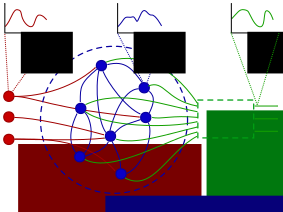
\includegraphics[width=0.6\textwidth]{figures/reservoir}
    \caption{High-level view of an echo state network RC.  An input
    signal (red, top left) drives an internal reservoir to produce a
    reservoir response (blue, top center) which is then combined to
    form an output signal (green, top right). In an ESN, the reservoir
    network has external input signals (red nodes, left) that drive
    the internal network (blue nodes, center) to produces an overall
    output (green, right).  Each internal node may have two kinds of
    input connections: connections to other nodes in the network
    ($W_r$, blue arrows), or connections to the overall input
    ($W_\text{in}$, red arrows). Each node may also contribute to the
    overall output ($W_\text{out}$, green arrows). Note that the
    internal connections may contain cycles.  When the ESN is used to
    perform forecasting, the output on the right side is connected to
    the input on the left side, allowing the ESN to run autonomously
    with no external input.}%
  \label{fig:reservoir}
\end{figure}

Put together, the dynamics of an echo state network RC are
\begin{align}
  \label{eq:esn}
  \dot{\bm{r}}(t) &= - \gamma \bm{r}(t) + \gamma \bm{f}\left( W_r\;\bm{r}(t) + W_\text{in}\;\bm{u}(t) \right), \\
  \bm{y}(t) &= W_\text{out}\;\bm{g}\left(\bm{r}(t)\right), \nonumber
\end{align}
where the vector function $\bm{f}$ is understood to mean applying the
one-dimensional activation function $f$ component-by-component. This
construction is summarized in \cref{fig:reservoir}. I will discuss
choosing the matrices $W_\text{in}$ and $W_r$, the parameter $\gamma$,
and the activation function $f$ in \cref{sec:esn-construction}.

This is the continuous-time formulation of an ESN. It is also common
to see a discrete-time formulation, which can be derived simply from
\cref{eq:esn} by the application of forward Euler
integration. Additionally, the forecasting method described in
\cref{sec:forecasting} involves a modification to the RC equation once
the RC is trained. These variations on the ESN equation are summarized
in \cref{tab:esn}.

\begin{table}
  \caption{A summary of variations of the ESN equation. The
    discrete-time formulation is the result of Euler-integrating the
    continuous-time formulation, and the forecasting variant is
    derived via the substitution described in \cref{sec:forecasting}.}
  \begin{tabular}{clrl}
    & Variation & & Equations \\
    \hline
    \rule{0pt}{4ex}
    (a) & Continuous & $\bm{\dot{r}}(t) =$ & $- \gamma \bm{r}(t) + \gamma \bm{f}\left( W_r\;\bm{r}(t) + W_\text{in}\;\bm{u}(t) \right)$ \\
    & (inference) & $\bm{y}(t) =$ & $W_\text{out}\;\bm{g}\left(\bm{r}(t)\right)$ \\
    \rule{0pt}{4ex}
    (b) & Continuous & $\bm{\dot{r}}(t) =$ & $- \gamma \bm{r}(t) + \gamma \bm{f}\left( W_r\;\bm{r}(t) + W_\text{in}\;W_\text{out}\;\bm{g}\left(\bm{r}(t)\right) \right)$ \\
    & (forecasting) & $\bm{y}(t) =$ & $W_\text{out}\;\bm{g}\left(\bm{r}(t)\right)$ \\
    \rule{0pt}{4ex}
    (c) & Discrete & $\bm{r}(t + \Delta t) =$ & $(1 - \gamma \Delta t) \bm{r}(t) + \gamma \Delta t \bm{f}\left( W_r\;\bm{r}(t) + W_\text{in}\;\bm{u}(t) \right)$ \\
    & (inference) & $\bm{y}(t + \Delta t) =$ & $W_\text{out}\;\bm{g}\left(\bm{r}(t + \Delta t)\right)$ \\
    \rule{0pt}{4ex}
    (d) & Discrete & $\bm{r}(t + \Delta t) =$ & $(1 - \gamma \Delta t) \bm{r}(t) + \gamma \Delta t \bm{f}\left( W_r\;\bm{r}(t) + W_\text{in}\;W_\text{out}\;\bm{g}\left(\bm{r}(t)\right) \right)$ \\
    & (forecasting) & $\bm{y}(t + \Delta t) =$ & $W_\text{out}\;\bm{g}\left(\bm{r}(t + \Delta t)\right)$ \\
  \end{tabular}
  \label{tab:esn}
\end{table}

% FIXME cite \gamma \Delta t = 1
The Euler integration is only an accurate representation of
\cref{eq:esn} when $\gamma \Delta t \ll 1$. However, many authors will
take $\gamma \Delta t = 1$. Although this is no longer an accurate
approximation to the continuous-time ESN in \cref{eq:esn}, these
discrete-time ESNs still function well as an RC. That the RC is not
sensitive to this kind of fundamental change in the underlying
reservoir is a hallmark of the RC method. The specific form of the
underlying reservoir is largely unimportant, except for a few
requirements to be discussed in
\cref{sec:reservoir-properties}. Indeed, the internal structure of an
ESN is determined randomly.

\section{Constructing ESNs}\label{sec:esn-construction}

The parameters $W_r$, $W_\text{in}$, $\gamma$, and $f$ in
\cref{eq:esn} must be set before the ESN construction is complete. Of
these, $\gamma$ has the most simple interpretation: it controls the
exponential decay of the value of each node in the network. As the
overall input to the ESN only influences the network via node inputs,
if this decay rate is too slow then the network will not be able to
react fast enough to its input to be useful for computing the
output. If instead this rate is too high, it is possible the network
will respond too quickly and have no memory of past inputs, which may
be necessary for the ESN's task.  The rate $y$ only controls the
dynamics of an individual node, however, and both of these effects can
be mitigated by the overall dynamics of the entire network of
nodes. For example, a network with very fast nodes may still retain
useful memory of past inputs if it contains long recurrent
loops. Network structure can also exacerbate a poor choice of
$\gamma$, as a network made of fast nodes that also contains very
short recurrent loops may begin to oscillate rapidly, which is
undesirable if the ESN's desired output does not contain such
oscillation.  In practice, this decay rate should be matched to the
characteristic timescale of the output signal, and then can be
manually tuned from there if needed.

If the read-out function $\bm{g}$ is taken to be the identity
function, as is common, and the activation function $f$ is linear,
then the forecasting-mode equations in \cref{tab:esn} are completely
linear and have simple, oscillatory analytic solutions. These are
known as \emph{linear ESNs}. Linear ESNs are mathematically easy to work
with, and as a result many of the known proofs about ESNs are in the
context of linear ESNs. One of the most recent and prominent results is
discussed further in \cref{ch:nvar}.

However, because the solutions to a linear ESN in prediction mode are
so simple, it is not possible for them to reproduce the strange
attractors of chaotic systems. To do this, the activation function $f$
is used to introduce nonlinearity into the equations. The most common
choice is the hyperbolic tangent, $f(x) = \tanh(x)$, and I will use this choice
in this dissertation. This satisfies the nonlinearity requirement, and
also ensures that each component of $\bm{r}(t)$ is bounded in $(-1,
1)$. Bounds on $\bm{r}(t)$ ensure that \cref{eq:esn} is particularly
well-behaved for numerical integrators. These bounds can also be used
to put bounds on the output $\bm{y}(t)$, which may be useful if that
output is driving a real-world system.

It is also possible to leave $f$ linear, and introduce nonlinearity
into the system with $\bm{g}$. These \emph{output-layer nonlinear ESNs} are
also discussed further in \cref{ch:nvar}.

The matrices $W_r$ and $W_\text{in}$, and therefore the topology and
weights of the ESN, are chosen randomly. There are many random schemes
in use, from Erd{\"{o}}s-R{\'{e}}nyi networks and small-world
networks~\cite{haluszczynski2019} to simpler cycle and line
networks~\cite{rodan2011}. The scheme I use is simple. Although this
dissertation only discusses RCs simulated in software, this scheme is
designed with an eye towards hardware implementation, where the number
of inputs to each node, and the total number of connections in the
network, have an associated hardware cost.

For the internal connections $W_r$, I generate a random network where
every node has a fixed number of inputs, or \emph{in-degree}, $k$. For
each node, I select $k$ nodes in the network without replacement and
use those as inputs to the current node. Each input is assigned a
random weight drawn from a normal distribution with mean $0$ and
variance $1$. This results in a connection matrix $W_r'$ where each
row has exactly $k$ non-zero entries. Finally, I rescale the whole
matrix by
\begin{equation}
  \label{eq:setradius}
  W_r = \frac{\rho_r}{\operatorname{SR}(W_r')}\;W_r',
\end{equation}
where $\operatorname{SR}(W_r')$ is the spectral radius, or maximum
absolute eigenvalue, of the matrix $W_r'$. This scaling ensures that
$\operatorname{SR}(W_r) = \rho_r$. This parameter is used to tune the
overall scale of the recurrent weights, and therefore the importance
of recurrent connections inside the network.

For $W_\text{in}$, I randomly connect each node to each RC input in
$\bm{u}(t)$ with probability $\sigma$. The weight for each connection
is drawn randomly from a normal distribution with mean $0$ and
variance $\rho_\text{in}^2$.

Together, $\sigma$ and $\rho_\text{in}$ are enough to generate a
random instantiation of $W_\text{in}$, and $k$ and $\rho_r$ are enough
to generate a random instantiation of $W_r$. The relative scales
$\rho_r$ and $\rho_\text{in}$ determine the importance of the
recurrent and external inputs, respectively. The entire ESN construction
is then reduced to choosing these \emph{meta-parameters}, summarized in
\cref{tab:esn-metaparameters}.

\begin{table}
  \caption{Summary of echo state network meta-parameters. These
    parameters must be chosen to produce a random realization of an
    ESN-based RC.}
  \begin{tabularx}{\linewidth}{rlX}
    & Parameter & Description \\
    \hline
    \rule{0pt}{4ex}
    $N$ & Number of Nodes & the total number of nodes in the network. \\
    \rule{0pt}{4ex}
    $\gamma$ & Leak Rate & controls the exponential decay of each node. \\
    \rule{0pt}{4ex}
    $\sigma$ & Input Connectivity & the probability that any given input is connected to any given node. \\
    \rule{0pt}{4ex}
    $\rho_\text{in}$ & Input Scale & the variance of the normally-distributed input connection weights. \\
    \rule{0pt}{4ex}
    $k$ & Recurrent Connectivity & the number of input connections each node draws from other nodes in the network. \\
    \rule{0pt}{4ex}
    $\rho_r$ & Recurrent Scale & the spectral radius of $W_r$. This controls the scale of recurrent connection weights. \\
    \rule{0pt}{4ex}
    $f$ & Activation Function & the function computed at each node. This is usually $\tanh$. \\
    \rule{0pt}{4ex}
    $\bm{g}$ & Read-out Function & the output layer read-out. This is usually the identity function. \\
    \rule{0pt}{4ex}
    $\alpha$ & Ridge Parameter & regularization parameter for ridge regression \\
  \end{tabularx}
  \label{tab:esn-metaparameters}
\end{table}

\section{Properties of Good Reservoirs}\label{sec:reservoir-properties}

Which dynamic systems make for good reservoirs, and what properties
are desired in a reservoir, remains an open question. There are a
handful of known desirable properties that are used to guide reservoir
design, and in particular ESN design. Chief among these is the
\emph{fading memory property}, also known as the echo state property, which states that the reservoir's
response to its input should have a vanishing dependence on the value
of that input signal in the distant past~\cite{jaeger2001,jaeger2002}.

More concretely, let $\bm{u}_1(t)$ and $\bm{u}_2(t)$ be two different
RC input signals which may differ for $t < 0$ but are otherwise
identical for $t > 0$, and let $\bm{r}_1(t)$ and $\bm{r}_2(t)$ be the
reservoir's response to these inputs. The reservoir has fading memory
if and only if $\bm{r}_1(t) \rightarrow \bm{r}_2(t)$ as $t \rightarrow \infty$.

This has many practical benefits for an RC. A reservoir with fading
memory guarantees a consistent output for a given input, regardless of
the path through state space the input takes in the distant past. This
is particularly important as running an RC often involves
resetting the internal reservoir, either in simulation or in
hardware. The fading memory property ensures that the specific initial
state of the reservoir does not matter, as long as it has a
sufficiently long warm-up time as discussed in \cref{sec:training}.

One early result for ESNs states that this fading memory property
cannot hold in an ESN when the input $\bm{u}(t) = 0$ and the spectral radius
of the matrix $W_r$ is greater than one~\cite{jaeger2001},
as any two distinct initial reservoir states
$\bm{r}_1(0)$ and $\bm{r}_2(0)$ must diverge exponentially as $t
\rightarrow \infty$.

Likewise, an ESN with $\operatorname{SR}(W_r) \ll 1$ is contracting,
and will return to $\bm{r} = 0$ rapidly with zero input. These two
considerations have combined in literature into a recommendation that
the spectral radius of $W_r$ be near, but not above,
one~\cite{lukosevicius2012}. However, both of these results only hold
for zero input, which is never the case when using an ESN in practice.
Once the ESN and the input system are considered as a single coupled
system, the ESN can display fading memory even when
$\operatorname{SR}(W_r) > 1$, and may never return to $\bm{r} = 0$
even when $\operatorname{SR}(W_r) \ll 1$.  More recent work presented
in \cref{ch:low-connectivity} and
elsewhere~\cite{pathak2017,rodan2011} show that these spectral radius
recommendations are not hard and fast rules. Nonetheless, this history
has cemented spectral radius as the standard measure of scale for
$W_r$ in ESNs.

Another desirable property of the reservoir is \emph{separability} and
\emph{continuity of response}. Similar inputs to the reservoir should produce
similar responses. This is especially important in real-world
applications, where the input to the RC is likely to be noisy. This
excludes a wide class of chaotic systems from consideration as a
reservoir, as even very small differences in two input signals would
be amplified. Likewise, a good reservoir should produce different
responses to different inputs. In the extreme case, a reservoir that
produces a constant zero regardless of input would form a very poor RC,
despite meeting the other criteria listed so far.

More recently, these requirements have been unified under the umbrella
of \emph{invertable generalized
  synchronization}~(IGS)~\cite{lu2018,lymburn2019,lu2020}, which claims that
a good reservoir is one that is synchronized to its
input. Specifically, the reservoir $\bm{r}(t)$ is in a state of
generalized synchronization with its input $\bm{u}(t)$ if there is a
function $\bm{H}$ such that, as $t \rightarrow \infty$, $\bm{r}(t)
\rightarrow \bm{H}\left(\bm{u}(t)\right)$. This already implies the
fading memory property. If $\bm{H}$ is continuous, this implies continuity of response, and if $\bm{H}$ is invertable, this implies separability. An invertable $\bm{H}$ also ensures that
\begin{equation}
  \bm{u}(t) \approx \bm{H}^{-1}\left(\bm{r}(t)\right).
\end{equation}
This is close to the form of the RC's output during forecasting in
\cref{eq:approx-output-forecast}, although there is no guarantee that
$\bm{H}^{-1}$ is linear.

The IGS approach differs from the earlier design principles in that it
considers the unified reservoir/input system together, rather than
looking for desirable properties of the reservoir
independently. Unfortunately, it yields very little actionable advice
about building a reservoir to use, and testing for the presence of IGS
in an RC computationally expensive. The quickest way to see if a
reservoir will work is still to build an RC with it, train it, and
test it. Nonetheless, this new approach unifies many older principles
in the field and is one of the most interesting avenues for future
research.

\section{Evaluating Reservoirs}

To evaluate the performance of a trained RC, it is common to use an
example testing input/output signal pair, $\bm{u}_\text{test}(t)$ and
$\bm{y}_\text{test}(t)$, that differs from the training signal. The
input $\bm{u}_\text{test}(t)$ is fed in to the trained RC, producing
the RC output $\bm{y}(t)$, which is then compared to the desired
output $\bm{y}_\text{test}(t)$. Note that the same concerns with
reservoir warm-up, as discussed in \cref{sec:training}, apply here: the
early part of the input test signal is used only to synchronize the
reservoir, and is not used in the comparison. Often, the training and
testing signals are combined such that $\bm{u}_\text{test}$ follows
directly after $\bm{u}_\text{train}$, which allows the training signal
to function as the warm-up signal for the reservoir during the testing
phase.

The most common metric for comparing the true output $\bm{y}(t)$ to
the desired output $\bm{y}_\text{test}(t)$ is to calculate the
normalized root-mean-square error (NRMSE) between them,
\begin{equation}
  \label{eq:nrmse}
  \epsilon = {\left(\sum_i\frac{\int \left| y_i(t) - y_{\text{test},i}(t) \right|^2 \;dt}{T \operatorname{Var}\left[y_{\text{test},i}(t)\right]}\right)}^{1/2},
\end{equation}
where the integral is evaluated on an interval of length $T$, and the
sum $i$ is over all components of $\bm{y}_\text{test}(t)$.  If
$\epsilon = 0$, then the two signals are identical during the interval
being evaluated, and any difference between them will result in
$\epsilon > 0$.

For RCs trained to do inference, this NRMSE is calculated across the
entire testing signal, regardless of length. However, for forecasting
this presents a problem. An RC in forecasting mode is autonomous,
after the warm-up period, and receives no ongoing external input as it
would in an inference task. The testing output may diverge quickly
from the reference system. Indeed, if the RC is trained to forecast a
chaotic system, good forecasting requires the forecast to diverge
eventually. In these situations, the testing error is calculated only
for a period of $T = 1/\lambda_\text{max}$, where $\lambda_\text{max}$
is the largest Lyapunov exponent of the system the RC is
forecasting. In this dissertation, I will refer to this one Lyapunov period
error as $\epsilon_1$.

Using $\epsilon_1$ as a testing metric for forecasting RCs is common,
but still has problems~\cite{pathak2017,haluszczynski2019}. The largest
issue is that the specific value of $\epsilon_1$ will depend strongly
on which specific input signal $\bm{u}_\text{test}(t)$ is used for
testing. If the input signal passes very near an unstable state of the
input system, very small errors in the RC's forecasting are amplified
dramatically. In these cases, $\epsilon_1$ is not a useful measure of
how well the RC has learned the input system. Examples of this are
given in \cref{ch:low-connectivity}.

\begin{figure}
  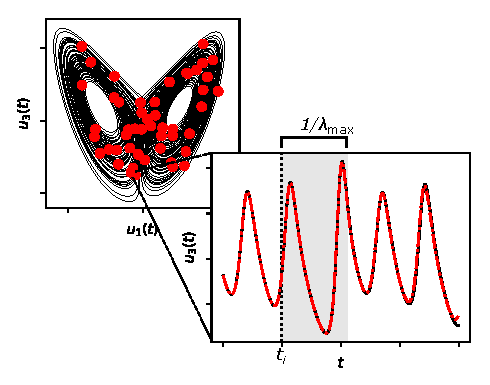
\includegraphics[width=0.6\textwidth]{figures/nrmse-avg}
  \caption{Summary of the forecasting evaluation method. I calculate
    errors $\epsilon_{1,i}$ at times $t_i$, marked on the attractor as
    red dots, and combine them into a single error
    $\tilde{\epsilon}$. Before each $t_i$ (dotted vertical line), the
    reservoir is integrated with \cref{eq:reservoir} and listening to
    the input. After $t_i$, the reservoir is integrated with
    \cref{eq:reservoir-auto}, and runs autonomously. The reservoir's
    prediction (dotted red line) must eventually diverge from the true
    system (solid black line). I calculate each $\epsilon_{1,i}$ only
    during a single Lyapunov period after forecasting begins, marked
    here in gray.}%
  \label{fig:nrmse-avg}
\end{figure}

To address these issues, I instead propose a new metric calculated from
$m$ forecasts with many different example inputs. I calculate an
$\epsilon_1$ value for each forecast, and then combine them into one
final metric
\begin{equation}
  \label{eq:nrmse-avg}
  \tilde{\epsilon} = {\left( \frac{1}{m} \sum_{i=1}^m \epsilon_{1,i}^2 \right)}^{1/2}.
\end{equation}
This method is summarized in \cref{fig:nrmse-avg}.
Using $\tilde{\epsilon}$ averages out the chance encounters with
unstable states, and as I will show in \cref{ch:low-connectivity}, is
a more reliable indicator of a forecasting RC's performance.

For forecasting, a very useful qualitative indicator of an RC's ability
to learn the input system is to use the RC in autonomous mode to
produce a very long forecast. This forecasted signal will necessarily
diverge from the true system, but both the forecast and the true
system can then be plotted side-by-side in state space. A well-trained
RC forecast will reproduce the shape of the input system's attractor,
and these plots can reveal immediate problems with the trained RC that
metrics like NRMSE sometimes mask. Still, this comparison is
completely qualitative -- it is imprecise, and not suitable to use in
an automated setting. Future research may develop a quantitative way
to measure the similarity between the RC's reconstructed attractor and
the true attractor, which would solve the problems with the current
NRMSE metric. In the meantime, visual inspection remains a useful
sanity check on the NRMSE.

\section{Summary}

Reservoir computers are a simple tool that uses an auxiliary dynamic
reservoir to transform its input. They can be trained on example data,
and that training is done very quickly using linear regression
tools. Once trained, RCs can be used in inference tasks, or in an
autonomous mode to perform system forecasting.

The RC approach is robust to the choice of reservoir system, however
the specific requirements the reservoir must have to function are
largely unknown. When an RC fails, it is difficult to know why. Recent
work on invertable generalized synchronization is an exciting path
towards learning more.

Echo state networks are a network-based reservoir choice that is easy
to simulate in software, and replicates more traditional neural
network machine learning designs. This approach uses several
meta-parameters to randomly construct the internal network. As with the
general reservoirs, there is not much concrete guidance on what values
these meta-parameters should have.

In \cref{ch:low-connectivity}, I will explore some of these
meta-parameters, and conclude that several guidelines for ESN
construction are not necessary. I will demonstrate several RCs with
very simple internal networks that nonetheless successfully replicate
the climate of a chaotic dynamic system.

\chapter{Low-Connectivity Reservoirs}\label{ch:low-connectivity}

The choice of ESN meta-parameters that best fits a given task is
difficult to identify. In the absence of strong guiding rules, a
practical approach is to treat it as an optimization problem. In this
chapter, I explore using ESNs on the chaotic system forecasting task,
for the Lorenz '63 system, the R{\"{o}}ssler system, and the
double-scroll circuit system described in \cref{ch:systems}. This
exploration is guided by optimization -- by trying to discover the
meta-parameters that result in the best averaged NRMSE
$\tilde{\epsilon}$ during forecasting for the given system. This
exploration leads to a surprising discovery, that even ESNs with
simple internal structure perform as well as their more complicated
siblings.

In particular, I am interested in the recurrent connectivity $k$. In
software simulations, such as those described in this thesis, the
connectivity $k$ has only a slight impact on the speed of the
simulation. However, in hardware network implementations, each
connection has an associated cost. For autonomous Boolean networks
implemented on FPGAs, every network connection is built from a long
chain of delay nodes.\cite{canaday2018} These delays often compose the
majority of the resource budget of the hardware network. Although the
results in this chapter are all software simulation, the particular
focus on the $k$ parameter is done with an eye towards hardware
implementations.

Many techniques have been used previously for ESN meta-parameter
optimization, such as grid search\cite{rodan2011} and gradient
descent\cite{jaeger2007}. However, both of these approaches have
drawbacks. Grid search quickly becomes intractable when the number of
dimensions grows, and even after fixing the two functional
meta-parameters $f$ and $\bm{g}$, there are 5 dimensions
left. Compounding this problem, the ESN construction is a random
process, and so the resulting measured $\tilde{\epsilon}$ for a given
set of meta-parameters is a random variable. To get a meaningful
result, each set of meta-parameters would need to be tested multiple
times. For even a coarse grid search, with 10 trials and 10 points per
meta-parameter, this already means one million trial RCs. Gradient
descent suffers from the randomness of ESN construction as well, for
the same reasons. It is also unsuitable for use with continuous
parameters such as $k$.

The problems with random ESN construction can be mitigated by
modifying the ESN construction method outlined in
\cref{sec:esn-construction} to front-load the random choices. For
example, once the recurrent weight matrix $W_r$ has been constructed,
the parameter $\rho_r$ can be changed without any random process at
all. By cleverly factoring out the random parts of ESN construction,
it becomes possible to use methods like grid search and gradient
descent without the extra step of multiple random trials. Ultimately,
however, this is optimizing only a single random instantiation of an
ESN, and provides little insight into how the fully random ESN will
perform.

In this chapter, I will be using Bayesian
optimization\cite{yperman2016,maat2018}, as implemented by the
\texttt{skopt} Python package\cite{skopt2018}, to explore which
meta-parameters result in the lowest forecasting error
$\tilde{\epsilon}$ for the three example systems. Bayesian
optimization deals well with both noise and integer parameters like
$k$, is more efficient than grid search,\cite{maat2018} and works well
with minimal tuning.

\section{Bayesian Optimization}

% FIXME cartoon figure for this?
Bayesian optimization is an optimization technique that finds the
minimum of an objective function $h(\bm{x})$ by repeated
evaluation. The process starts with a prior distribution of functions,
representing the algorithm's knowledge of the function $h$. As each
new point $\bm{x}$ is evaluated, the algorithm incorporates this new knowledge
and updates its prior distribution. At the start of the optimization,
points are chosen randomly. This is the exploration phase, where the
Bayesian optimizer is only gathering data to improve it's prior
distribution. After exploration, the optimizer will then evaluate
points $\bm{x}$ with the most expected improvement over the best known minimum
so far.

This algorithm has a number of drawbacks. Primarily, it is
complicated. The above summary only scratches the surface, and already
suggests a number of parameters to the optimization algorithm that can
be tuned, such as the initial prior distribution of functions. This
complication makes it difficult to directly claim that any minimum
found is the true minimum, and so I emphasize that this algorithm is
used here for exploration. I am interested in ESNs that perform well,
and what they have in common, but not in claiming any ESN as the best
performer possible. For this purpose, the unopinionated defaults of
the \texttt{skopt} package suffice.

The complexity of this optimization algorithm also manifests in run
time. After the exploration phase, calculating the next set of trial
parameters $\bm{x}$ involves minimizing an internal function
calculated from the current prior distribution. This can be quite
computationally expensive, and so Bayesian optimization is only
suitable for use when the objective function $h(\bm{x})$ is expensive
enough to justify the extra work to reduce how often it is
evaluated. This makes it a good fit for minimizing prediction error
$\tilde{\epsilon}$ as this involves building, training, and testing
an RC each time.

\begin{table}
  \caption{Range of meta-parameters searched using Bayesian optimization.}
  \begin{tabular}{lrcl}
    Parameter & min & & max \\
    \hline
    $\gamma$ & 7 & -- & 11 \\
    $\sigma$ & 0.1 & -- & 1.0 \\
    $\rho_\text{in}$ & 0.3 & -- & 1.5 \\
    $k$ & 1 & -- & 5 \\
    $\rho_r$ & 0.3 & -- & 1.5 \\
  \end{tabular}%
  \label{tab:bayes-ranges}
\end{table}

In this chapter, the Bayesian algorithm repeatedly generates a set of
meta-parameters to test within the ranges listen in
\cref{tab:bayes-ranges}. Larger ranges would require a longer
optimization time. I selected these ranges to include values that
existing ESN design heuristics would choose, while also allowing
exploration outside those ranges without a prohibitively long runtime.

During the optimization process, I discovered that the optimizer was
often finding ESNs with $k = 1$ that perform as well as ESNs with a
higher $k$. Such networks have an interesting and simple network
structure, and also suggest other simple structures for comparison.

\section{Structure of Low-Connectivity Reservoirs}

First, networks generated with $k = 1$ often have multiple
disconnected components. For higher $k$, this is still possible but
relatively rare, as $k$ controls the number of opportunities for
components in the network to connect. Disconnected components in the
network essentially act as ESNs operating in parallel. This is an
interesting line of research,\cite{pathak2018} but not one I
investigate further here. In the interest of a more equitable
comparison between $k = 1$ networks and $k > 1$, I discard and
regenerate any networks with more than a single connected component.

\begin{figure}
  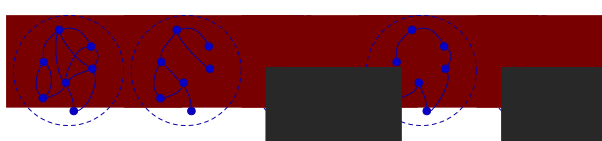
\includegraphics[width=\textwidth]{figures/topology}
  \caption{The five reservoir structures tested. Only internal
    reservoir connections are pictured. Connections to the reservoir
    computer input, or to the output layer are not shown. (a) A
    general, fixed in-degree network, here pictured with $N=7$ and
    $k=2$. (b) A $k=1$ network with a single connected component. (c)
    A $k=1$ network with the single cycle cut at an arbitrary
    point. (d) A \emph{simple cycle reservoir}. (e) A \emph{delay line
      reservoir}.}%
  \label{fig:topology}
\end{figure}

A $k = 1$ network with only a single connected component must also
contain only a single directed cycle. Starting from any node in the
network and working backwards through the single input connection each
node must have will always lead to a single directed cycle, and it is
not possible for two such cycles to exist in the network unless they
are disconnected from each other. This severely limits how recurrence
can occur inside a $k = 1$ network compared to higher-$k$
networks. Every node in a $k = 1$ network is either part of this core
cycle, or part of a directed tree branching off from this cycle, as
depicted in \cref{fig:topology}~(b).

Inspired by the high performance of this simple structure, I also
investigate $k = 1$ networks when the single cycle is cut at a random
point. This turns the entire network into a tree, as in
\cref{fig:topology}~(c).

Finally, I also investigate reservoir networks that consist entirely
of a cycle or a ring with identical weights with no attached tree
structure, depicted in \cref{fig:topology}~(d), and networks with a
single line of nodes (a cycle that has been cut), in
\cref{fig:topology}~(e). These choices were inspired by the $k = 1$
networks, but have also been researched previously and are known as
\emph{simple cycle reservoirs} and \emph{delay line reservoirs},
respectively.\cite{rodan2011}

In total, there are five network structures I investigate:
\begin{enumerate}[label= (\alph*)]
\item general construction with unrestrained $k$,
\item $k = 1$ with a single cycle,
\item $k = 1$ with a cut cycle,
\item single cycle, or \emph{simple cycle reservoir},
\item single line, or \emph{delay line reservoir}.
\end{enumerate}
Both the $k = 1$ cut cycle networks (c) and line networks (e) are
rescaled to have a fixed $\rho_r$ before the cycle is
cut. However, after the cycle is cut, they both have $\rho_r=0$.

\section{RC Symmetries and their Consequences}

An ESN in autonomous forecast mode, described by \cref{tab:esn}~(b),
has an inversion symmetry about the origin. That is, if $\bm{r}(t)$ is
a solution to this equation, so is $-\bm{r}(t)$. For an output layer
with an identity read-out function $\bm{g}$, this means that if
$\bm{y}(t)$ is a possible output of the trained RC, then so is
$-\bm{y}(t)$. If the underlying system the RC was trained to forecast
also exhibits this symmetry, this is not a problem. In fact, designing
the internal reservoir to match symmetries with the input system can
dramatically improve RC performance\cite{barbosa2021}.

However, if the input system does not have this symmetry, this can be
an issue. If at any time the autonomous forecast strays near $\bm{r} =
0$, the solution can hop over the symmetry to the other side, and
begin producing an output $\bm{y}(t)$ that is flipped through the
origin. This problem is exacerbated if the input signal $\bm{u}(t)$ is
normalized to have mean zero, a common practice.

This problem was identified early, and a common fix\cite{pathak2017,herteux2020}
is to use a non-linear read-out function
\begin{equation}
  g_i(\bm{r}) = \begin{cases}
    r_i & \text{if } i \leq N / 2, \\
    r_i^2 & \text{if } i > N / 2.
  \end{cases}
  \label{eq:esn-break-sym}
\end{equation}
This squares half of the node values before being passed
to the output layer, and breaks the inversion symmetry in the ESN
equation while keeping the number of features accessible to the output
layer the same.

%score: 0.08873905001779689
%score-1: 0.007877037205449461
\begin{figure}
  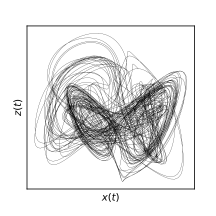
\includegraphics[width=0.6\textwidth]{figures/lorenz-symmetry}
  \caption{The forecasted attractor from an ESN trained on the Lorenz
    '63 system, with identity read-out, in the $x$/$z$ plane. Compare
    against \cref{fig:lorenz}, and note the two deformed images of the
    butterfly attractor on top of each other, with one flipped along
    the $z$ axis.}
  \label{fig:lorenz-symmetry}
\end{figure}

This problem can be difficult to diagnose if the input system has a
partial inversion symmetry. For example, the Lorenz '63 system in
\cref{eq:lorenz} has an $(x, y) \rightarrow (-x, -y)$ symmetry, and so the
complete inversion of the Lorenz attractor looks exactly the same as a
flip along the $z$ axis. This is misleading, as the problem has
nothing to do with the Lorenz $z$ variable specifically, and this
confusion prevented a full understanding of the problem until
recently.\cite{herteux2020} \cref{fig:lorenz-symmetry} provides an
example of the forecasting failure characteristic to the identity
read-out function.

For consistency, I use this \emph{quadratic read-out} for all three
example input systems, even if the inversion symmetry exists in the
input system as it does for the double-scroll circuit.

\section{Training, Forecasting, and Evaluation}

Now that I have identified the five networks structures of interest, I
can use the Bayesian optimization algorithm to identify networks in
each class that perform well on the system forecasting task. I
optimize the meta-parameters independently for each of the three
example input systems: Lorenz '63 (\cref{sec:lorenz}), R{\"{o}}ssler
(\cref{sec:rossler}), and the double-scroll circuit
(\cref{sec:dscroll}).

For each input system and for each network structure, the Bayesian
algorithm performs random exploration for $50$ iterations, and then
optimization for $50$ iterations, resulting in $100$ iterations in
total. At each iteration of the algorithm, the optimizer constructs a
single random instantiation of an ESN with the chosen meta-parameters,
trains it, and measures its forecasting performance with the metric
$\tilde{\epsilon}$ defined in \cref{eq:nrmse-avg}. Since the
exploration phase of the optimization is random, I repeat this entire
process 20 times to estimate the variance in the performance of
reservoirs optimized by this method.

To ensure that results are comparable across all three systems, I
normalize their components to have $0$ mean and unit variance. In
addition, I rescale the time axes of all systems so that their maximum
positive Lyapunov exponent matches that of the Lorenz system,
$\lambda_\text{max} = 0.9056$.

To train the ESN, I integrate \cref{eq:esn} with the quadratic readout
in \cref{eq:esn-break-sym}, coupled with the chosen input system, via
the hybrid Runge-Kutta~5(4)\cite{dormand1980} method from $t = 0$ to
$300$. This produces an ESN response $\bm{r}(t)$. I then divide this interval into three ranges:
\begin{itemize}
\item $t = 0$ -- $100$: the warm-up period,
\item $t = 100$ -- $200$: the training period,
\item $t = 200$ -- $300$: the testing period.
\end{itemize}
As discussed in \cref{sec:training}, the warm-up period is used to
ensure the later times do not depend on the specific initial
conditions of the ESN. I divide the rest into a training period, used
only during training, and a testing period, used later only to
evaluate the ESN performance.

I then determine $W_\text{out}$ via ridge regression, as in
\cref{eq:ridge}, where the sum ranges over the training period. The
ridge parameter $\alpha$ could be included among the meta-parameters to
optimize. However, unlike the other meta-parameters, modifying $\alpha$
does not require re-integration and can be optimized with simpler
methods. I select an $\alpha$ from among $10^{-5}$ to $10^5$ by
leave-one-out cross-validation. This method also reduces the number of
dimensions the Bayesian algorithm must work with.

To evaluate the performance of the trained ESN, I use it to perform
autonomous forecasting using \cref{tab:esn}~(b). I choose $50$ times
$t_i$ spaced evenly within the testing period. For each $t_i$, I
initialize the reservoir state to $\mathbf{r}(t_i)$, and then
integrate forward with the autonomous equation for one Lyapunov
period, between $t = t_i$ and $t = t_i + 1 / \lambda_\text{max}$. This
produces a reservoir forecast during these times, from which I
calculate an error $\epsilon_{1,i}$ as described in
\cref{eq:nrmse}. Finally, I combine these $50$ errors into a single
$\tilde{\epsilon}$, as in \cref{eq:nrmse-avg}, that represents the
average ability of the ESN to forecast accurately at any point on the
input system attractor.

\begin{figure}
  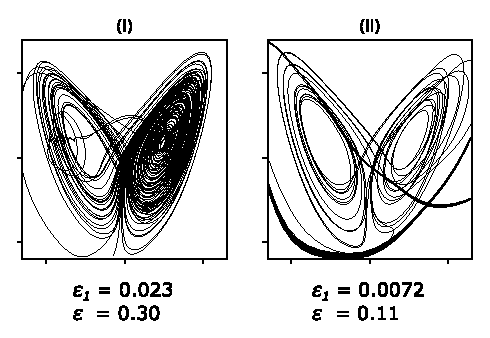
\includegraphics[width=0.6\textwidth]{figures/epsilon-failure}
  \caption{Two examples of reservoir computers that fail to reproduce
    the Lorenz attractor, but produce a low $\epsilon_1$. Compare with
    the true attractor in \cref{fig:lorenz}. Reservoir (i) fails to
    learn the attractor, overemphasizing the right lobe in which $t_1$
    resides. Reservoir (ii) matches the attractor well early on, but
    as the prediction lengthens, it falls into a periodic orbit (thick
    black line). Both (i) and (ii) show a promising low $\epsilon_1$,
    but the averaged $\tilde{\epsilon}$ measure more accurately
    captures their failure to learn the Lorenz attractor.}%
  \label{fig:epsilon-failure}
\end{figure}

Using $\tilde{\epsilon}$ and not simply $\epsilon_1$ is even more
important in an optimization setting, as searching for ESNs with the
lowest $\epsilon_1$ risks producing ESNs that are only good at
forecasts near $t_1$, but otherwise perform poorly in reproducing the
attractor of their input system. It can also waste time, as the
optimization algorithm explores areas of the parameter space it
believes perform well, but actually do not. \Cref{fig:epsilon-failure}
depicts two common ways for an RC to fail to replicate the true Lorenz
attractor, shown in \cref{fig:lorenz}. However, both produce a good
short-term forecast near $t_1$. In particular, reservoir (ii) in
\cref{fig:epsilon-failure} has a lower $\epsilon_1$ than any of
the optimized reservoirs despite its obvious failure to learn the
Lorenz attractor.

\section{Results}

First, I run all five reservoir structures through 100 iterations of
the Bayesian algorithm using the Lorenz system as input, and record
the best-performance RC for each structure according to the metric
$\tilde{\epsilon}$. These reservoirs, and the meta-parameters that
generated them, are reported in \cref{tab:lowk-lorenz-results}. I
estimate the errors on these with the standard deviation of
$\tilde{\epsilon}$ after repeating the optimization process 20 times.

\begin{table}
  \caption{Best reservoir computers of each reservoir structure, after 100
    iterations of the Bayesian optimization algorithm using the Lorenz
    system as input.  The meta-paremeters chosen by the algorithm are
    shown on the right. The simpler structures (b) -- (e) all perform
    nearly as well as the general structure (a).}
  \begin{tabularx}{\linewidth}{l l@{\extracolsep{\fill}} l d d d d}
    & & \multicolumn{5}{l}{Lorenz} \\
    & Structure & $\tilde{\epsilon}$ & \multicolumn{1}{c}{$\gamma$} & \multicolumn{1}{c}{$\sigma$} & \multicolumn{1}{c}{$\rho_\text{in}$} & \multicolumn{1}{c}{$\rho_r$} \\
    \hline
    (a) & Any $k$ \footnote{After optimization, $k = 3$.} & 0.022 $\pm$ 0.004 & 7.7 & 0.81 & 0.37 & 0.41 \\
    (b) & $k = 1$ with cycle & 0.024 $\pm$ 0.005 & 10.9 & 0.44 & 0.30 & 0.30 \\
    (c) & $k = 1$ no cycle & 0.028 $\pm$ 0.005 & 7.2 & 0.78 & 0.30 & 0.30 \footnote{\label{fn:lowk-rhor}$\rho_r$ measured before cycle is cut. Afterwards, $\rho_r = 0.$} \\
    (d) & cycle & 0.023 $\pm$ 0.008 & 7.9 & 0.17 & 0.58 & 0.30 \\
    (e) & line & 0.024 $\pm$ 0.003 & 10.6 & 0.79 & 0.30 & 0.45 \footref{fn:lowk-rhor} \\
  \end{tabularx}
  \label{tab:lowk-lorenz-results}
\end{table}

When optimized, all reservoir structures perform well. In particular,
the simpler structures all perform almost as well as the general-$k$
structure. They often lie within one, or at most two standard
deviations from structure (a). This is despite the fact that
structures (c) and (e) both have $\rho_r=0$ and no recurrent
connections within the network. The other structures have
$\rho_r\ll1$.  Previous work has already demonstrated that ESNs with
low or zero spectral radius can still
function.\cite{pathak2017,rodan2011} These results act as additional
counterexamples to the heuristic that ESNs should have $\rho_r \approx
1$.\cite{lukosevicius2012}

However, these best-observed ESNs are not representative of a
typical ESN.\@ I use the meta-parameters to guide the random input
connections and connections within the network, and so even once the
meta-parameters are fixed, constructing the network is a random
process. Not all networks with a fixed structure type and meta-parameters
will perform the same.

To explore this variation, I generate and evaluate $200$ networks of
each structure on the Lorenz system, using the optimized
meta-parameters in \cref{tab:lowk-lorenz-results}. For all five
structures, as the measured $\tilde{\epsilon}$ increases, the quality
of the reproduced attractor decreases gradually. On manual inspection
of the attractors, the reason for this decrease can be divided into
three qualitative regions. For $\tilde{\epsilon} < 0.3$, the RCs
reproduce the Lorenz attractor consistently. Failures still rarely
occur, but they always reproduce part of the attractor before falling
into a fixed point or periodic orbit. In this region, small
differences between the true attractor and the reproduced attractor
contribute more to $\tilde{\epsilon}$ than outright failure. For $0.3
< \tilde{\epsilon} < 1.0$, RCs always fail to reproduce the attractor,
though they will still always reproduce a portion of it before
failing. Examples of these failures are provided in
\cref{fig:epsilon-failure}. Above $\tilde{\epsilon} > 1.0$, these
failures become catastrophic, and no longer resemble the Lorenz
attractor at all. A more quantitative description of these regions is
one line of possible future research.

Though the optimized best-performing networks of
each structure show very little performance difference, the differences
between them become more apparent when we compare the probability
distribution of $\tilde{\epsilon}$ for each topology. These
distributions are shown in \cref{fig:epsilon-distribution}.

\begin{figure}
  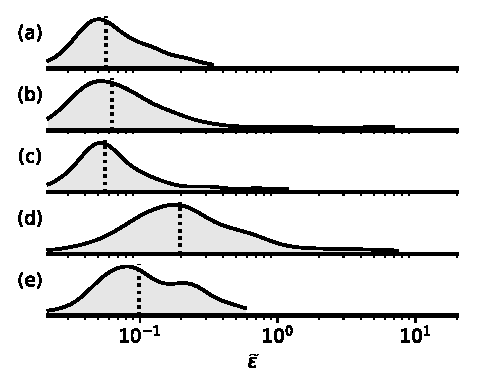
\includegraphics[width=0.6\textwidth]{figures/epsilon-distribution}
  \caption{Performance for each network structure, evaluated for the
    Lorenz system at the meta-parameters listed in
    \cref{tab:lowk-lorenz-results}. Each is visualized as a Gaussian
    kernel density estimation in $\log_{10} \tilde{\epsilon}$ with a bandwidth
    of 0.35,\cite{scott1992} which can be interpreted as a probability
    distribution. Using a narrower bandwidth does not reveal
    additional features. A vertical line marks the median.  Note that
    structures (b) -- (e) have very long tails, and can produce
    networks that perform very poorly in comparison to (a). However,
    all five have the capability to produce well-performing
    networks.}%
  \label{fig:epsilon-distribution}
\end{figure}

A well-performing network with arbitrary $k$ (a) is a much more
likely outcome than a well-performing network with a single cycle
(d). However, the performance of arbitrary $k$ networks (a) is very
similar to that of tree-like networks (c). Though (c) has a longer
tail on the high end, the simpler structure of the reservoir may be
appealing for hardware RCs.

The distribution of performance for each structure can be a deciding
factor if network construction and evaluation is expensive, as it
might be in hardware. In software, though, I find the
best-performing networks in \cref{tab:lowk-lorenz-results} after only $100$
trials. A hardware design can still benefit from the simpler
structures (b) -- (e) despite their very wide performance distributions
if the creation of the evaluation of the design can be automated to
test many candidate reservoirs, as on an FPGA.\cite{canaday2018}

There may also be a benefit in software. The simpler structures are
represented by weight matrices $W_r$ in very simple forms. Structure
(c) can always be represented as a strictly lower-diagonal matrix, and
(d) -- (e) can be represented with non-zero entries only directly below
the main diagonal. Software simulations can take advantage of this structure to
speed up integration of \cref{eq:esn}.

To explore whether these structures remain equally effective at tasks
beyond forecasting the Lorenz system, I run all five network
structures through 100 iterations of the Bayesian algorithm for both
the R{\"{o}}ssler and the double-scroll systems. As with the Lorenz
system, I estimate the errors on these results by repeating the
process 20 times each. These results are reported in
\cref{tab:lowk-resultsplus}.

\begin{table}
  \caption{Result of optimizing reservoirs with the
      Bayesian algorithm over 100 iterations, on both the
      R{\"{o}}ssler system and the double-scroll system. All five
      structures can perform equally well at both systems.}
  \begin{tabularx}{\linewidth}{l l@{\extracolsep{\fill}} l l}
    & & \multicolumn{1}{l}{Double Scroll} & \multicolumn{1}{l}{R{\"{o}}ssler} \\
    & Structure & $\tilde{\epsilon}$ & $\tilde{\epsilon}$ \\
    \hline
    (a) & Any $k$ & 0.029 $\pm$ 0.006 & 0.017 $\pm$ 0.005 \\
    (b) & $k = 1$ with cycle & 0.033 $\pm$ 0.007 & 0.020 $\pm$ 0.007 \\
    (c) & $k = 1$ no cycle & 0.033 $\pm$ 0.008 & 0.018 $\pm$ 0.006 \\
    (d) & cycle & 0.033 $\pm$ 0.007 & 0.018 $\pm$ 0.006 \\
    (e) & line & 0.037 $\pm$ 0.01 & 0.019 $\pm$ 0.015
  \end{tabularx}
  \label{tab:lowk-resultsplus}
\end{table}

The results for the double-scroll and R{\"{o}}ssler systems agree well
with those for Lorenz. All five structures optimize reliably with the
Bayesian algorithm, and all perform similarly when
optimized. Optimizing a network to reproduce either system will almost
always work after only 100 iterations, regardless of networks
structure.

\begin{figure*}
  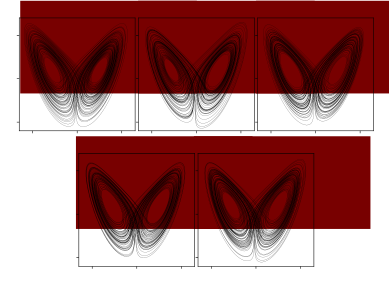
\includegraphics[width=\textwidth]{figures/lowk-attractors}
  \caption{Lorenz attractor plots in the $x$/$z$ plane for long-term
    free-running predictions for each network structure in
    \cref{tab:lowk-lorenz-results}. Compare with true Lorenz attractor
    in \cref{fig:lorenz}, and the failed reservoirs in
    \cref{fig:epsilon-failure}.}%
  \label{fig:lowk-attractors}
\end{figure*}

Finally, for each structure I produced a free-running prediction of
the Lorenz system for $100$ time units using the best-performing RC.\@
I use these predictions to produce an attractor as shown in
\cref{fig:lowk-attractors}. All five optimized ESNs reproduce the
Lorenz attractor well. Though comparing these plots by eye is not
quantitative, I find them qualitatively useful: an RC that fails to
reproduce the Lorenz attractor by eye is unlikely to have a low
$\tilde{\epsilon}$ compared to one that does, but visual inspection of
the reproduced attractor can catch rare catastrophic failures that are
not reflected in $\tilde{\epsilon}$.

\section{Cross-task Performance}

One advantage to RCs is that a single reservoir can be re-used on many
different tasks by re-training $W_{\text{out}}$. To evaluate whether
this is possible with these optimized networks, I take the 20 networks
optimized for the Lorenz system and re-train $W_{\text{out}}$ for each
to instead reproduce the double-scroll circuit system. Every other
part of the RC is left unchanged. I then evaluate how accurate this
prediction is using the metric $\tilde{\epsilon}$. These results are
summarized in \cref{tab:lowk-resultsgen}.

\begin{table}
  \caption{Result of re-using reservoirs optimized for
      Lorenz prediction to perform double-scroll prediction. The
      minimum error encountered across all 20 reservoirs of each
      topology is reported as $\tilde{\epsilon}_{\text{min}}$.}
  \begin{tabularx}{\linewidth}{l l@{\extracolsep{\fill}} l l}
    & & \multicolumn{2}{l}{Double Scroll} \\
    & Topology & $\tilde{\epsilon}$ & $\tilde{\epsilon}_\text{min}$ \\
    \hline
    (a) & Any $k$ & 0.43 $\pm$ 1.2 & 0.028\\
    (b) & $k = 1$ with cycle & 0.30 $\pm$ 0.5 & 0.048 \\
    (c) & $k = 1$ no cycle & 0.37 $\pm$ 0.8 & 0.032 \\
    (d) & cycle & 0.17 $\pm$ 0.2 & 0.056 \\
    (e) & line & 0.22 $\pm$ 0.3 & 0.058
  \end{tabularx}
  \label{tab:lowk-resultsgen}
\end{table}

In general, these reservoirs perform poorly on this new task. However,
there is extremely high variation. Even though they were optimized to
perform Lorenz forecasting, many of these reservoirs are still able to
reproduce the double-scroll attractor. Moreover, the best performers
in each category approach the performance of reservoirs optimized
specifically for the double-scroll system. This indicates that it is
possible to find a single reservoir in any of these topologies that
works well on more than one system. The Bayesian optimization
algorithm may be able to find these reservoirs more reliably if the
metric $\tilde{\epsilon}$ is modified to reward RCs that perform well
on many systems.

\section{Conclusion}

I find that Bayesian optimization of RC meta-parameters is a useful
tool for creating high-performance ESNs quickly. I also find
that allowing the optimizer to explore areas of the parameter space
that are typically excluded in other optimization studies can lead to
interesting and effective ESN designs such as those presented
here.

For this procedure to be effective, I find that evaluating the RC
performance at many points along the attractor and averaging, rather
than at a single point, encourages the optimization algorithm to find
networks that reproduce the climate of the input system. Using this
evaluation method helps direct the optimizer away from reservoirs that
perform good short-term forecasting at only one point on the input
system attractor.

One surprising outcome of our optimization procedure is finding
reservoirs that perform well even with no recurrent connections and
$\rho_r=0$.  Though some reservoirs of this kind have been explored
previously and shown to work,\cite{pathak2017,rodan2011} the
heuristics remain common in reservoir design. I present additional
concrete examples that provide evidence these heuristics are not
unbreakable rules.

In greater detail, I find reservoir networks with very low internal
connectivity that perform at least as well as their
higher-connectivity counterparts. A network with only a single
internal cycle, or even no cycle at all, can perform as well as those
with many recurrent cycles. These simpler structures manifest as
simpler weight matrices, which can result in faster integration in
software. In a hardware environment where connections between nodes
have a cost, or recurrence is difficult to implement, these network
structures may also have a direct benefit.

Though the best of these low-connectivity networks perform as well
as the more complicated reservoirs, they also tend to perform worse on
average. However, searching for the best-performing instance of these
reservoirs can be done in few trials, and may be feasible for hardware
reservoirs that can be constructed and evaluated in an automated way.

During this work, I have discovered many interesting lines of future
research. First, the metric $\tilde{\epsilon}$ can be evaluated by
comparing the output of the reservoir predictions to the true system
attractor using a new metric for attractor overlap.\cite{ishar2019}
This overlap metric can also be used to quantify the qualitative
observations of different failure modes in regions of the
$\tilde{\epsilon}$ metric. Second, these results show that these very
low connectivity reservoirs perform well in the narrow context of
software-based, chaotic system forecasting. Future work can explore
whether these results hold for other reservoir computing tasks such as
classification, and whether it is possible to find reservoirs that
perform well on a variety of tasks simultaneously by modifying the
metric $\tilde{\epsilon}$ to encourage generalization. Third, these
results may also generalize to RCs with hardware networks, where the
simpler reservoir designs would allow for more efficient and faster
operating hardware RCs.

At the time the work in this chapter was conducted, there were known
results that prove that a linear network architecture with
time-independent nodes, the discrete-time NARX networks, can simulate
fully-connected networks.\cite{siegelmann1997} A similar proof for RCs
would explain why there is no difference in the best-performing
reservoirs in each structure type. The discovery that a line network
(e) can perform as well as a general-$k$ network suggests that the
network's role in the RC may only be to produce a variety of time
delays for the output layer to draw on.

In the time since, such a proof has been discovered. In the next
chapter, I will introduce non-linear vector auto-regressions (NVARs),
an existing machine learning tool that is proven to be mathematically
equivalent to ESNs under specific conditions, and discuss how this
relationship between NVARs and RCs has advanced the understanding and
application of both.

\chapter{RCs without Reservoirs: Nonlinear Vector Auto-regressions}\label{ch:nvar}

In 2021, Erik Bollt proved~\cite{bollt2021} that a completely linear
ESN is mathematically equivalent to an existing tool known as a \emph{vector
auto-regression}, or VAR. He subsequently proved that an ESN with a
quadratic output nonlinearity is likewise equivalent to a
\emph{nonlinear VAR}, or NVAR.

In this chapter, I provide a brief outline of this equivalence proof,
beginning with a discussion of the behavior of fully linear ESNs as
well as their drawbacks. Later, I describe the VAR and NVAR
methods. This provides background information and motivation for the
original work presented in \cref{ch:nvar-application}.

Although output-nonlinear ESNs and NVARs are mathematically
equivalent, the conditions of their equivalence raise some practical
concerns when it comes to implementation. In this chapter discuss
these concerns, as well as the relative merits of the ESN and NVAR
approaches. In addition, I discuss how the NVAR approach benefits from
reinterpretation within the RC framework.

In \cref{ch:nvar-application} I build on the information provided
here to demonstrate the NVAR approach in practical applications, and
address these concerns about the applicability of Bollt's proof.

\section{Solutions to Linear ESNs}

\subsection{Prediction}

A fully linear ESN, with both the activation function $f$ and the
read-out function $\bm{g}$ set to the identity function, has very
simple solutions. 
As an example, I will take the discrete-time linear
ESN equation in prediction mode from \cref{tab:esn}~(d),
\begin{align}
  \bm{r}(t + \Delta t) &= (1 - \gamma \Delta t) \bm{r}(t) + \gamma \Delta t \left( W_r\;\bm{r}(t) + W_\text{in}\;W_\text{out}\;\bm{r}(t)\right), \label{eq:nvar-esn-forecast} \\
  \bm{y}(t+\Delta t) &= W_\text{out}\;\bm{r}(t+\Delta t).
\end{align}
The linear coefficients of $\bm{r}(t)$ can be collected into a single matrix
\begin{equation}
  W \equiv (1 - \gamma \Delta t) I + \gamma \Delta t \left( W_r + W_\text{in}\;W_\text{out}\right),
\end{equation}
simplifying the \cref{eq:nvar-esn-forecast} to
\begin{equation}
  \bm{r}(t + \Delta t) = W\;\bm{r}(t).
  \label{eq:nvar-esn-forecast-simple}
\end{equation}
Almost all square matrices of complex numbers are diagonalizable. If
$W$ is an $N \times N$ matrix, diagonalizing $W$ yields $N$
uncoupled time evolution equations $r_i(t + \Delta t) = w_i\;
r_i(t)$ where $w_i$ may be complex. Solutions to this equation are very simple,
\begin{equation}
  r_i(k \Delta t) = w_i^k\; r_i(0).
\end{equation}

This means the dynamics of the ESN amount to discrete-time complex
waves, possibly with an exponential growth or decay over time. This is
all the RC output layer has to draw from to construct the output
$\bm{y}(t)$. For the forecasting task, a sum of sine waves of
different frequencies can perform adequately well for short-term
prediction~\cite{bollt2021}, as this effectively amounts to a discrete
Fourier approximation. However, for long term attractor reconstruction
and the reproduction of global properties of the input system, this
linear ESN \emph{must} eventually fail on anything but the simplest
input system. The most direct demonstration of this failure is that
this linear ESN cannot predict any fixed point of the input system
except $\bm{y}(t) = 0$. It is possible to shift this fixed point to
another location by adding a constant term to
\cref{eq:nvar-esn-forecast-simple}, but this change can only move the
fixed point around, not add new ones.

To have any hope of reconstructing the underlying system attractor, as
demonstrated with ESNs in \cref{ch:low-connectivity}, an ESN must have some nonlinear component, either in the
activation function $f$ or the read-out function
$\bm{g}$. Still, a completely linear ESN is mathematically easy to
work with, and indeed the RC/NVAR equivalence proof begins by looking
at the behavior of a discrete-time linear ESN in inference mode.

\subsection{Inference}

For ESNs in inference mode, from \cref{tab:esn}~(c),
\begin{align}
  \bm{r}(t + \Delta t) &= (1 - \gamma \Delta t) \bm{r}(t) + \gamma \Delta t \left( W_r\;\bm{r}(t) + W_\text{in}\;\bm{u}(t) \right), \label{eq:nvar-esn} \\
  \bm{y}(t+\Delta t) &= W_\text{out}\;\bm{r}(t+\Delta t). \label{eq:nvar-esn-output}
\end{align}
The coefficients of $\bm{r}(t)$ and $\bm{u}(t)$ can be collected into two matrices,
\begin{align}
  A &\equiv (1 - \gamma \Delta t) I + \gamma \Delta t W_r, \\
  B &\equiv \gamma \Delta t W_\text{in}.
\end{align}
\Cref{eq:nvar-esn} then simplifies to
\begin{equation}
  \bm{r}(t + \Delta t) = B\;\bm{u}(t) + A\;\bm{r}(t).
\end{equation}
This equation is recursive; expanding it out into the past yields
\begin{align}
  \bm{r}(t + \Delta t) &= B\;\bm{u}(t) + AB\;\bm{u}(t - \Delta t) + A^2\;\bm{r}(t), \\
  \bm{r}(t + \Delta t) &= \sum_{j = 0}^\infty A^j B \bm{u}(t - j \Delta t). \label{eq:esn-var-mat}
\end{align}

\Cref{eq:esn-var-mat} states that the value of $\bm{r}(t + \Delta t)$
is constructed from a linear combination of time-delay taps of the
input $\bm{u}(t)$, extending infinitely into the past.  In combination
with \cref{eq:nvar-esn-output}, this means the overall output
$\bm{y}(t)$ is a linear combination of time-delay taps of the input
$\bm{u}(t)$.  This is known as a vector auto-regression.

\section{Linear Vector Auto-regressions (VARs)}

In most cases, the term \emph{vector auto-regression} specifically
means a method of producing an output $\bm{y}(t)$ from a linear
combination of past outputs. However, I generalize this slightly
to better mirror the reservoir computer model introduced in
\cref{ch:reservoir-computing}.

In this dissertation, a vector auto-regression (VAR) is a method of
transforming a discrete-time input signal $\bm{u}(t)$ into a
discrete-time output signal $\bm{y}(t)$ from a linear combination of
time-delay taps. Given a list of tap delays $\tau_i$, I construct
a tap vector $\bm{v}(t)$ via
\begin{equation}
  \label{eq:var-v}
  \bm{v}(t + \Delta t) = \bm{u}(t - \tau_0 \Delta t) \oplus \bm{u}(t - \tau_1 \Delta t) \oplus \cdots \oplus \bm{u}(t - \tau_{q-1} \Delta t)
\end{equation}
where the operator $\oplus$ is understood to mean vector
concatenation. That is, if the input $\bm{u}(t)$ has dimension $d$,
and if there are $q$ taps, then the vector $\bm{v}(t)$ has dimension
$dq$. Most commonly, $\tau_0 = 0$, which ensures that the VAR has access to the most recent information from $\bm{u}(t)$ when producing an output.

\begin{figure}
  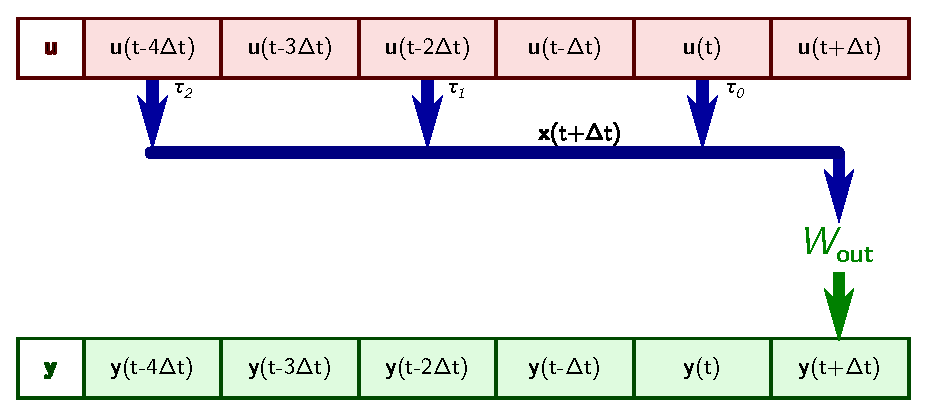
\includegraphics{figures/var-infer}
  \caption{Summary of the (N)VAR method. Many time-delay taps $\tau_i$
    of the discrete-time signal $\bm{u}(t)$ (top, red) are concatenated into the tap
    vector $\bm{v}(t)$ (middle, blue). Here, there are three taps
    $\tau_0=0$, $\tau_1=2$, and $\tau_2=4$. These taps are then passed
    through a possibly nonlinear function $\bm{g}_\text{n}$ and
    combined linearly by the output matrix $W_\text{out}$ to produce
    the next value of the (N)VAR's output $\bm{y}(t)$ (bottom,
    green). For a linear VAR, $\bm{g}_\text{n}$ is the identity
    function. To transform a whole time series input, this (N)VAR process
    slides along the time axis from left to right.}
  \label{fig:var-infer}
\end{figure}

The output of the VAR is the linear transformation of this tap vector by the matrix $W_\text{out}$,
\begin{equation}
  \label{eq:var-y}
  \bm{y}(t + \Delta t) = W_\text{out}\;\bm{g}_\text{n}\left(\bm{v}(t + \Delta t)\right),
\end{equation}
where $\bm{g}_\text{n}$ is the identity function. If $\bm{g}_\text{n}$
is instead chosen to be nonlinear, this results in a nonlinear VAR,
which I discuss in \cref{sec:nvar}.

This transformation process, from input to output, is summarized in
\cref{fig:var-infer}. Note the similarity to the RC method: the input
signal $\bm{u}(t)$ drives an internal state $\bm{v}(t)$ / $\bm{r}(t)$,
which is then linearly transformed into the output
$\bm{y}(t)$. However, the internal state $\bm{v}(t)$ of the VAR is
much simpler than that of most reservoirs, because it is constructed
directly from the input.

\subsection{Training and Testing}

Once the taps $\tau_i$ are selected, the VAR can be trained in much
the same way as an RC. The VAR is fed an example input
$\bm{u}_\text{train}(t)$, which produces an example tap vector
$\bm{v}_\text{train}(t)$ via \cref{eq:var-v}. Finally, a $W_\text{out}$
that best maps this $\bm{v}_\text{train}(t)$ onto the example output
$\bm{y}_\text{train}(t)$ can be found via ridge regression, exactly as
in the RC case.

VARs can also be used for forecasting as well. Analogously to the RC
case, the VAR used for forecasting can be trained to reproduce the
example input as its output. Since the VAR output $\bm{y}(t + \Delta
t)$ depends only on $\bm{u}(t)$ at time $t$ and earlier, this amounts
to one step ahead prediction. Once trained, the VAR can do autonomous
prediction by replacing the input $\bm{u}(t)$ with the output
$\bm{y}(t)$ in \cref{eq:var-v}.

For practical reasons, in this dissertation, forecasting VARs have a modified
output equation
\begin{equation}
  \bm{y}(t + \Delta t) = \bm{u}(t) + W_\text{out}\;\bm{g}_\text{n}\left(\bm{v}(t + \Delta t)\right).
\end{equation}
This effectively changes the VAR from one step ahead prediction to
predicting the difference between the last value of the signal and the
next, in analogy to a discrete-time integrator. Without this change,
the components of $W_\text{out}$ corresponding to $\bm{u}(t)$ are
larger than the others. Because the ridge regression used to find
$W_\text{out}$ has a single regularization parameter $\alpha$, it
works best when all components of $W_\text{out}$ have about the same
expected scale.

Once trained, either as a signal transformation or for prediction, a
VAR can be tested in the same ways as an RC. For signal
transformations, the VAR output is compared to the true signal,
yielding a NRMSE $\epsilon$. For prediction, the VAR can be used to
generate multiple predictions for a single Lyapunov time, and the
NRMSE $\epsilon_1$ from these predictions is combined into an average
error $\tilde{\epsilon}$.

\subsection{Comparing VARs to ESNs}

Working with a VAR, by training it and using it, is very similar to
working with an RC. The most important difference is that using a VAR
completely sidesteps the issue of choosing an internal
reservoir. Building an ESN reservoir is a complicated process that
starts with the meta-parameters listed in
\cref{tab:esn-metaparameters} and ends with a random realization of a
network, usually of 100 nodes or more. In contrast, building a VAR
amounts to selecting which taps $\tau_i$ to use, and how many. This
dramatic reduction in the parameter space makes VARs easier to build
and use, and the lack of a random component makes it possible to
deterministically specify a VAR's construction.

By describing the VAR method within the reservoir computing framework,
there are a few benefits to the VAR method as well. Previous work with
VARs has trained the $W_\text{out}$ matrix with least squares, while
work in the RC field has long used ridge regression as a way to reduce
overfitting and encourage generalization. In addition, VARs benefit
from the more sophisticated forecasting evaluation methods, such as
$\tilde{\epsilon}$, developed for use with RCs.

However, the linear ESN solution in \cref{eq:esn-var-mat} is only
completely equivalent to a VAR with an infinite number of time delay
taps. VARs with a finite number of taps $q$ approximate a VAR
with infinite taps under the right conditions as $q \rightarrow
\infty$~\cite{bollt2021}, but if VARs are to be used as a replacement
for RCs, it is critical to know how good this approximation is in
practice. If a VAR requires thousands of taps to work, it may still
be simpler just to use an ESN.

Finally, these linear VARs suffer from the same drawbacks as the
linear ESN. Any practical replacement for a full, nonlinear ESN would have to
reproduce the attractors of the systems they are trained on, as in
\cref{ch:low-connectivity}, and to do that, they need a nonlinearity.

\section{Nonlinear Vector Autoregressions (NVARs)}\label{sec:nvar}

The ESN model has two possible sources of nonlinearity: the
activation function $f$ and the read-out function $\bm{g}$. Most
commonly, including in \cref{ch:low-connectivity}, $f =
\tanh$. However, a nonlinear $f$ is mathematically difficult to work
with, as it lies in the middle of the ESN's internal state equation. In
contrast, the read-out function $\bm{g}$ sits only on the output
layer. Consider the linear ESN described in
\cref{eq:esn-var-mat} modified to have a nonlinear read-out function
\begin{equation}
  g_i(\bm{r}) = \begin{cases}
    r_i & \text{if } i \leq N, \\
    r_{i - N}^2 & \text{if } N < i \leq 2N.
  \end{cases}
  \label{eq:esn-quadratic-out}
\end{equation}
where $N$ is the number of nodes in the ESN.  That is,
$\bm{g}(\bm{r})$ contains all of the node values, as well as the
square of all the node values. This is similar to the read-out
function used in \cref{ch:low-connectivity}, except that it makes no
attempt to keep the dimension of $\bm{g}(\bm{r})$ the same as the dimension of $\bm{r}$. By
\cref{eq:esn-var-mat}, each node value is a linear combination of
time-delay taps of $\bm{u}(t)$, and so the square of a node value
contains only quadratic terms of the form $u_i(t-j\Delta
t)u_k(t-l\Delta t)$.

Putting this together, the ESN's output $\bm{y}(t)$ can written in
terms of the time-delay tap vector $\bm{v}(t)$ in \cref{eq:var-v},
using an infinite number of taps $\tau_i = i$,
\begin{equation}
  \bm{y}(t + \Delta t) = W_\text{out}\;\bm{g}_\text{n}\left(\bm{v}(t + \Delta t)\right).
\end{equation}
The nonlinear function $\bm{g}_\text{n}(\bm{v})$ has all
components of $\bm{v}$ as well as all quadratic pairs of those components,
\begin{equation}
  \label{eq:quadratic-nvar}
  \bm{g}_\text{n}(\bm{v}) = \bm{v} \oplus \ceil{\bm{v} \otimes \bm{v}}.
\end{equation}
Here, the operator $\otimes$ denotes the outer product, and $\ceil{X}$
denotes the a flattened vector that contains the upper-triangular
components of $X$. For example, $\ceil{\bm{v} \otimes \bm{v}}$ is a
vector that contains as components all unique terms of the form $v_i
v_j$.

This construction, a VAR that wraps the delay tap vector in a
nonlinear function $\bm{g}_\text{n}$ before the building the linear
combination for the output, is known as a nonlinear VAR (NVAR). This
concludes a sketch of Bollt's proof that a linear ESN with quadratic
read-out is mathematically equivalent to an NVAR with infinite
taps~\cite{bollt2021}. Because the read-out function appears only on
the output, it is not difficult to change the nature of the nonlinear
read-out $\bm{g}$ in an ESN and derive the corresponding NVAR $\bm{g}_\text{n}$,
and therefore this proof generalizes easily to read-out functions that are more
complicated than quadratic.

It is important to note at this point that the ESN's output weights
$W_\text{out}$ and read-out $\bm{g}$ are \emph{not} the same as the
equivalent NVAR's output weights $W_\text{out}$ and nonlinearity
$\bm{g}_\text{out}$. In this example, the ESN's $\bm{g}$ produces node values and squares of node
values, while the NVAR's $\bm{g}_\text{n}$ produces all linear and
quadratic terms it is possible to construct from the tap vector
$\bm{v}$. The NVAR has quadratic terms that mix both the dimensions of the input $\bm{u}(t)$ as well as mix the tap delays $\tau_i$. In a practical application with a finite tap vector, this
means that if $\bm{v}$ has $q$ taps and $\bm{u}$ is dimension $d$, then $\bm{g}_\text{n}$ will have
$qd + qd(qd+1)/2$ components. This quadratic dependence on $qd$ can
rapidly cause the computational cost of the ridge regression to find $W_\text{out}$ to be very
expensive, as either the number of taps or the input dimension increases.

Putting all the pieces together, the NVAR method for transforming an
input $\bm{u}(t)$ into an output $\bm{y}(t)$ is described by
\begin{align}
  \label{eq:nvar}
  \bm{v}(t + \Delta t) &= \bm{u}(t - \tau_0 \Delta t) \oplus \bm{u}(t - \tau_1 \Delta t) \oplus \cdots \oplus \bm{u}(t - \tau_{k-1} \Delta t), \\
  \label{eq:nvar-out}
  \bm{y}(t + \Delta t) &= W_\text{out}\;\bm{g}_\text{n}\left(\bm{v}(t + \Delta t)\right).
\end{align}
For forecasting tasks, the output \cref{eq:nvar-out} is replaced with
\begin{equation}
  \label{eq:nvar-out-forecast}
  \bm{y}(t + \Delta t) = \bm{u}(t) + W_\text{out}\;\bm{g}_\text{n}\left(\bm{v}(t + \Delta t)\right).
\end{equation}

Simply by wrapping the tap vector $\bm{v}$ in a nonlinear function
before the output, the NVAR now has the nonlinearity required to have
any hope of reproducing attractors as well as the nonlinear ESNs, and
in \cref{ch:nvar-application} I demonstrate that NVARs perform
quite well in this role.

\section{Practical Considerations}

The above sketch of Bollt's proof demonstrates that a linear ESN with nonlinear
readout is equivalent to an NVAR with an infinite number of taps. In
practice, though, this method can only be implemented with a finite
number of taps. If an NVAR implementation requires thousands of taps
to work, it is not a realistic replacement for the ESN method.

The number of taps $q$ and input dimension $d$ are also relevant for the quadratic
$\bm{g}_\text{n}$ described in \cref{eq:quadratic-nvar}. The output
dimension of this function, $qd + qd(qd + 1)/2$, is also one of the
dimensions of the output matrix $W_\text{out}$. As this dimension
grows, so does the time required to perform ridge regression. This
quadratic dependence on $q$ also emphasizes the need to keep the
number of taps low.

On top of this, a quadratic output may not be enough. If a quadratic
NVAR is trained to do forecasting on a system with total inversion
symmetry $\bm{u}(t) \rightarrow -\bm{u}(t)$, the quadratic terms in
the output cannot meaningfully contribute. This reduces the NVAR to a
linear VAR, with all the forecasting problems that entails. To use an
NVAR on such a system, the nonlinear function $\bm{g}_\text{n}$ must
be expanded to include higher-order terms. This can be done by
constructing an ESN and calculating the equivalent NVAR form, but it
can also be done more directly by simply adding higher-order monomial terms to
$\bm{g}_\text{n}$. I explore this in
\cref{ch:nvar-application}. However, this further emphasizes the
requirement for a small number of taps, as the number of terms of
order $n$ grows as $(qd)^n$.

\begin{table}
  \caption{Summary of NVAR parameters. Compared to the ESN approach in
    \cref{tab:esn-metaparameters}, the NVAR method is much simpler.}
  \begin{tabularx}{\linewidth}{rlX}
    & Parameter & Description \\
    \hline
    \rule{0pt}{4ex}
    $\tau_i$ & Tap Delays & the placement of time-delay taps \\
    \rule{0pt}{4ex}
    $\bm{g}_\text{n}$ & Read-out Function & the nonlinearity on the output layer \\
    \rule{0pt}{4ex}
    $\Delta t$ & Time Step & the discrete time step of both the input $\bm{u}(t)$ and the NVAR itself \\
    \rule{0pt}{4ex}
    $\alpha$ & Ridge Parameter & regularization parameter for ridge regression \\
  \end{tabularx}
  \label{tab:nvar-parameters}
\end{table}

If these challenges can be overcome, NVARs are an extremely appealing
replacement for the ESN approach. ESNs are complicated random networks
with many poorly-understood meta-parameters. In contrast, NVARs have
only four total parameters, listed in \cref{tab:nvar-parameters}.  In
addition to being a smaller set of parameters, these parameters are
simply much more interpretable. It is not straightforward to imagine
what changing the input connectivity of an ESN will do to performance,
but changing the taps $\tau_i$ has a direct effect on what information
is available to the NVAR.

\section{Summary}

VARs and NVARs are, like RCs, a method of transforming an input signal
into an output signal. They operate on linear combinations of
time-delay taps of the input. In many ways, their construction and use
mirrors that of an RC, except that there is no internal dynamic
reservoir system. This sidesteps a whole host of questions and
decisions relating to reservoir construction, and dramatically
simplifies the implementation of VARs and NVARs. However, despite this
simplicity, they are now known to be mathematically equivalent to an
output layer nonlinear ESN.

NVARs are an existing method, but they are not widely used or discussed. This equivalence opens the door
to cross-talk between the NVAR and RC communities. On the RC side,
researchers gain a dramatically simpler implementation that is known
to be equivalent, and also gain a chance to apply lessons learned in
the RC world to the NVAR method. The NVAR approach benefits from the
use of ridge regression, long used in the RC field, instead of other
linear fitting methods.  It also benefits from improvements to
evaluation, such as $\tilde{\epsilon}$, and opens the door to using
NVARs on traditional RC problems. However, some questions still
remain -- most notably, how many time-delay taps are practically
necessary, and how complicated a nonlinear function will most tasks
need?

If these questions are resolved, the NVAR approach is an extremely
attractive alternative to the ESN approach. NVARs do not rely on
random construction, are simple to implement, and have only a few
parameters with direct interpretations. If NVARs work well, it becomes
difficult to recommend ESNs and the complications they entail.

In the next chapter, I apply the NVAR method to the traditional
RC tasks of system state inference and chaotic system forecasting. In
the process, I resolve these remaining questions, and demonstrate
that NVARs are a practical and very simple replacement for traditional
ESN approaches.

\chapter{NVARs in Practice}\label{ch:nvar-application}

In this chapter, I resolve the practical questions raised in
\cref{ch:nvar}, and demonstrate that NVARs are capable of solving
traditional RC problems well with very few taps, simple
nonlinearities, and very little training data. Using the example
systems from \cref{ch:systems}, I use NVARs to perform state
inference and forecasting on the Lorenz '63 system, forecasting on the
double-scroll circuit, and forecasting on the Mackey-Glass time-delay
system.

The work presented in this chapter is the result of a
collaboration with Daniel~J.~Gauthier, Erik~Bollt, and Wendson~A.S.~Barbosa~\cite{gauthier2021}. My contribution involves the initial
implementation and exploration of the NVAR method, discussion during
the development of the Lorenz '63 results, as well as
implementing the Lorenz return map, double-scroll forecasting,
and Mackey-Glass forecasting.

\section{State Inference with Lorenz '63}

For this inference task, I provide an NVAR with the $x$ and $y$
components of the Lorenz '63 system, and train it to infer the third
$z$ variable. Inference tasks like this are useful in situations where
some variables of a system are easily measurable, while the rest are
only measurable with great care or expense. For example, a mechanical
engine can be outfitted at great expense with a large array of
internal temperature and pressure sensors, and an NVAR can be trained
to infer these variables from easily-accessible external sensors. Once
trained, the NVAR can now be reused on engines manufactured without
the expensive internal instrumentation.

To build an NVAR, I must choose the time-step $\Delta t$, the tap
delays $\tau_i$, the nonlinearity $\bm{g}_\text{n}$, and ridge
parameter $\alpha$. For this task, I use an integration time-step of
$\Delta t = 0.05$. Takens' embedding theorem~\cite{takens1981}
provides guidance on the expected number of taps: as the dimension of
the Lorenz attractor is slightly larger than $2$, I choose to use $4$
equally spaced taps $\tau_0 = 0$, $\tau_1 = 5$, $\tau_2 = 10$, and
$\tau_3 = 15$. These taps are spaced to equally cover roughly one
Lyapunov period, with the last tap at time $\tau_3 \Delta t = 0.75$.

For the nonlinearity $\bm{g}_\text{n}$, I use a slightly modified
version of the quadratic output introduced in
\cref{eq:quadratic-nvar}. This $\bm{g}_\text{n}$ includes a constant
term, all linear terms of the tap vector $\bm{v}$, and all quadratic
terms of the tap vector $\bm{v}$. That is,
\begin{equation}
  \label{eq:quadratic-nvar-const}
  \bm{g}_\text{n}(\bm{v}) = 1 \oplus \bm{v} \oplus \ceil{\bm{v} \otimes \bm{v}}.
\end{equation}
The addition of a constant term allows the trained linear
$W_\text{out}$ to fit a constant offset, which is useful here as the
$z$ component is always positive, even when both $x$ and $y$ are zero.
For this task, with $q = 4$ taps and $d = 2$ input dimensions, $x$ and $y$, the
output of $\bm{g}_\text{n}$ has $1 + 8 + 36 = 45$ components, and the linear
output matrix $W_\text{out}$ has dimension $1 \times 45$.

\begin{figure}
  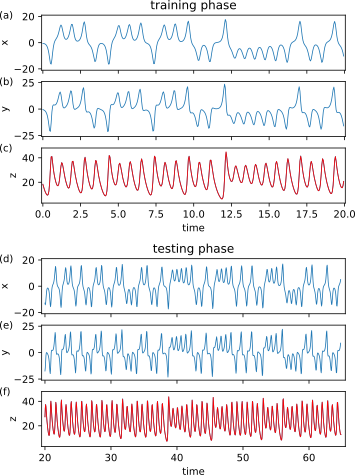
\includegraphics{figures/nvar-infer-lorenz}
  \caption{(a) -- (c) The Lorenz '63 system (blue) during the NVAR
    training. After the NVAR is trained, it is re-used on the
    training signal to produce the training output (c, red). (d) --
    (f) The Lorenz '63 system during NVAR testing, with the NVAR
    output. In both cases, the NVAR output (red) lies directly on top
    of the true Lorenz signal (blue).}
  \label{fig:nvar-infer-lorenz}
\end{figure}

I train this NVAR on $10$ different examples of the Lorenz '63
system, using $x$ and $y$ as the example input and $z$ as the example
output. Each training example is $20$ time units ($400$ data points). I then evaluate
the NVAR for $45$ time units ($900$ data points) to produce a NRMSE $\epsilon$ as in
\cref{eq:nrmse}, and then average these errors over all $10$
trials. During evaluation, the NVAR has access to only $x$ and $z$,
and must produce an estimate of $z$. I then adjust $\alpha$ manually
to minimize this error. This whole process, training the NVAR $10$
different times and evaluating the error, takes only a few seconds on
a modern computer even with a poorly-optimized implementation.

I find this NVAR has a NRMSE of $1.75\mp0.3\times10^{-2}$ on this
inference task, using the ridge parameter $\alpha = 0.05$. An example
of the NVAR during a single training and testing trial is shown in
\cref{fig:nvar-infer-lorenz}. The trained NVAR shows good agreement in
the $z$ component during both the training phase (c) and the testing
phase (f); in fact, the agreement is so good that when the NVAR signal is
drawn on top of the true Lorenz signal, the true signal is not visible
underneath.

\subsection{Output Weights}\label{sec:nvar-infer-weights}

The output weights $W_\text{out}$ from a single trial, visualized in
\cref{fig:nvar-infer-lorenz-wout}, have two notable features. First,
the largest trained weight by far corresponds to the $1$ term in
$\bm{g}_\text{n}$. This accounts for the fact that $z$ is always
positive, and justifies the inclusion of the constant term in
$\bm{g}_\text{n}$.

\begin{figure}
  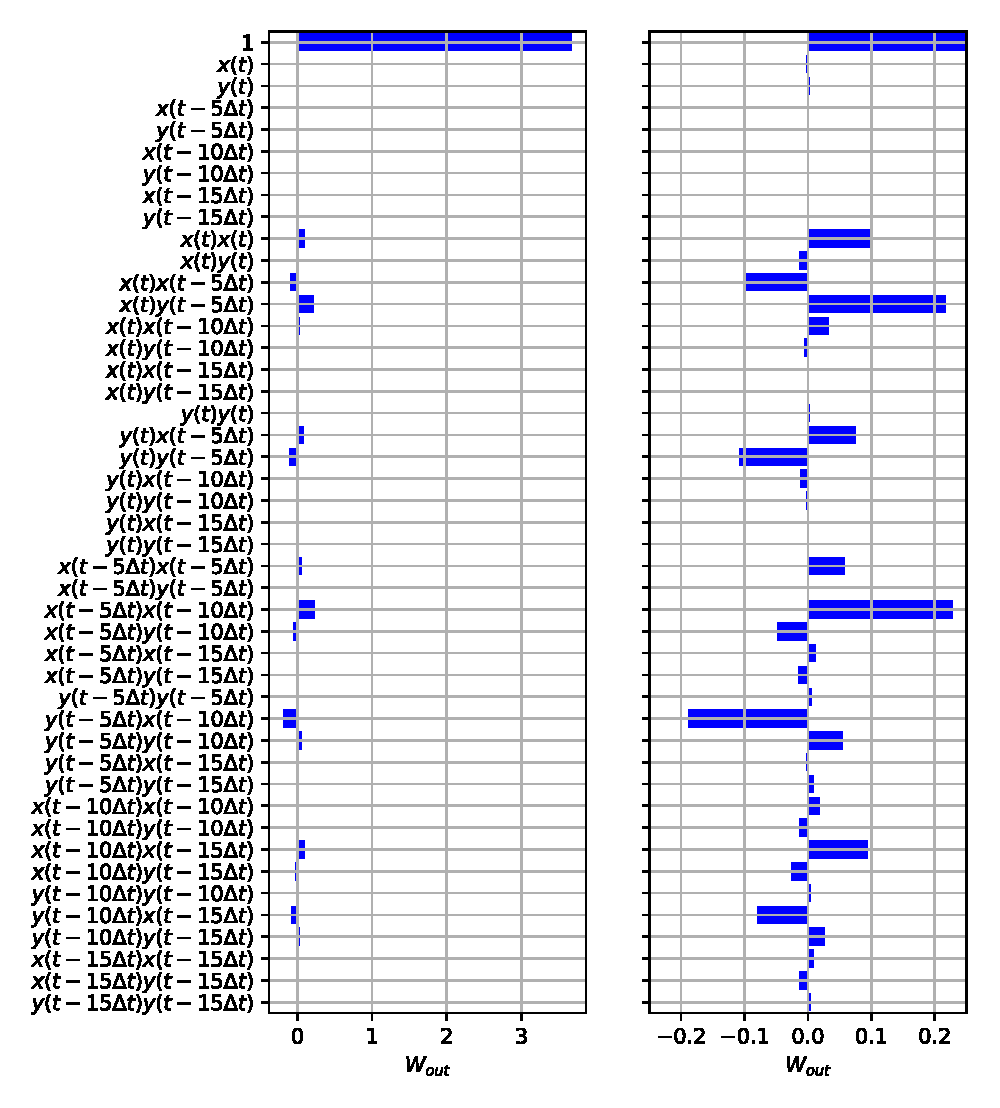
\includegraphics[width=\textwidth]{figures/nvar-infer-lorenz-wout}
  \caption{Weights in the matrix $W_\text{out}$ (left) for the NVAR
    trained for Lorenz system forecasting. On the right, a magnified
    view of the same. The largest component is the constant offset, to
    account for the fact that the $z$ component of the Lorenz system
    is positive, even when both $x$ and $y$ are zero. Also note that
    the linear terms in $x$ and $y$ (highlighted in red) have weights near zero. As the
    Lorenz system has a $(x, y) \rightarrow (-x, -y)$ symmetry, the
    NVAR must have zero weights attached to these terms to respect
    that symmetry.}
  \label{fig:nvar-infer-lorenz-wout}
\end{figure}

Second, the weights of all the linear terms in $x$ and $y$ are all
near zero. This reflects the $(x, y) \rightarrow (-x, -y)$ symmetry of
the Lorenz system. Since the NVAR input $\bm{u}(t)$ is just these $x$
and $y$ terms, in order to respect this symmetry the NVAR must predict
the same $z(t)$ for both $\bm{u}(t)$ and $-\bm{u}(t)$. This is only
possible if the linear terms in $x$ and $y$ have zero coefficients.

In general, an NVAR does not need to respect any symmetries not
present in the training input. Specifically, if the NVAR is trained on only a small
part of the input system's phase space, it does not need to respect
symmetries outside that space to perform well within that space. Here,
however, the NVAR training input $\bm{u}_\text{train}(t)$ overlaps
with its symmetric counterpart $-\bm{u}_\text{train}(t)$, and so
learning the example input necessarily means learning the symmetry.

Later, in \cref{sec:nvar-mackey-glass}, I will investigate a task
where the example input does not overlap with its symmetric
counterpart, and demonstrate that the NVAR will learn weights that do
not agree with this symmetry.

\section{Forecasting Lorenz '63}

For this task, I use an NVAR in forecasting mode to do system
forecasting for the Lorenz '63 system. That is, I train the NVAR to
use all three state variables $x$, $y$, and $z$ to perform
next-step-ahead prediction of the Lorenz system in
\cref{eq:lorenz}. Unlike for the inference task, the NVAR has no
external driving input and runs autonomously once it is in forecast
mode. In analogy to other discrete-time integration algorithms, the
choice of time step $\Delta t$ has a stronger effect on forecasting
than inference. Too small a time step is wasted effort, and too large
risks inaccuracy. Here, I use a time step of $\Delta t = 0.025$, which
results in about $40$ steps per Lyapunov period.

For this forecasting task, I use only $2$ taps, $\tau_0 = 0$ and
$\tau_1 = 1$. That is, the NVAR has access to the two previous time
steps, and I find this is enough for the forecasting task.  I use the
quadratic nonlinearity with constant term described in
\cref{eq:quadratic-nvar-const}. With $q = 2$ taps and $d = 3$ input dimensions,
the nonlinear output of $\bm{g}_\text{n}$ has $1 + 6 + 21 = 28$
components, and so $W_\text{out}$ has dimension $3 \times 28$.

Again, I train this NVAR on $10$ different examples of the Lorenz '63
system, each time training on $10$ time units ($400$ data points). I then evaluate the
NVAR by performing an autonomous forecast for one Lyapunov period to
calculate a NRMSE $\epsilon_1$, as in \cref{eq:nrmse}, and then
average this over the $10$ trials to produce $\tilde{\epsilon}$ in
\cref{eq:nrmse-avg}.

\begin{figure}
  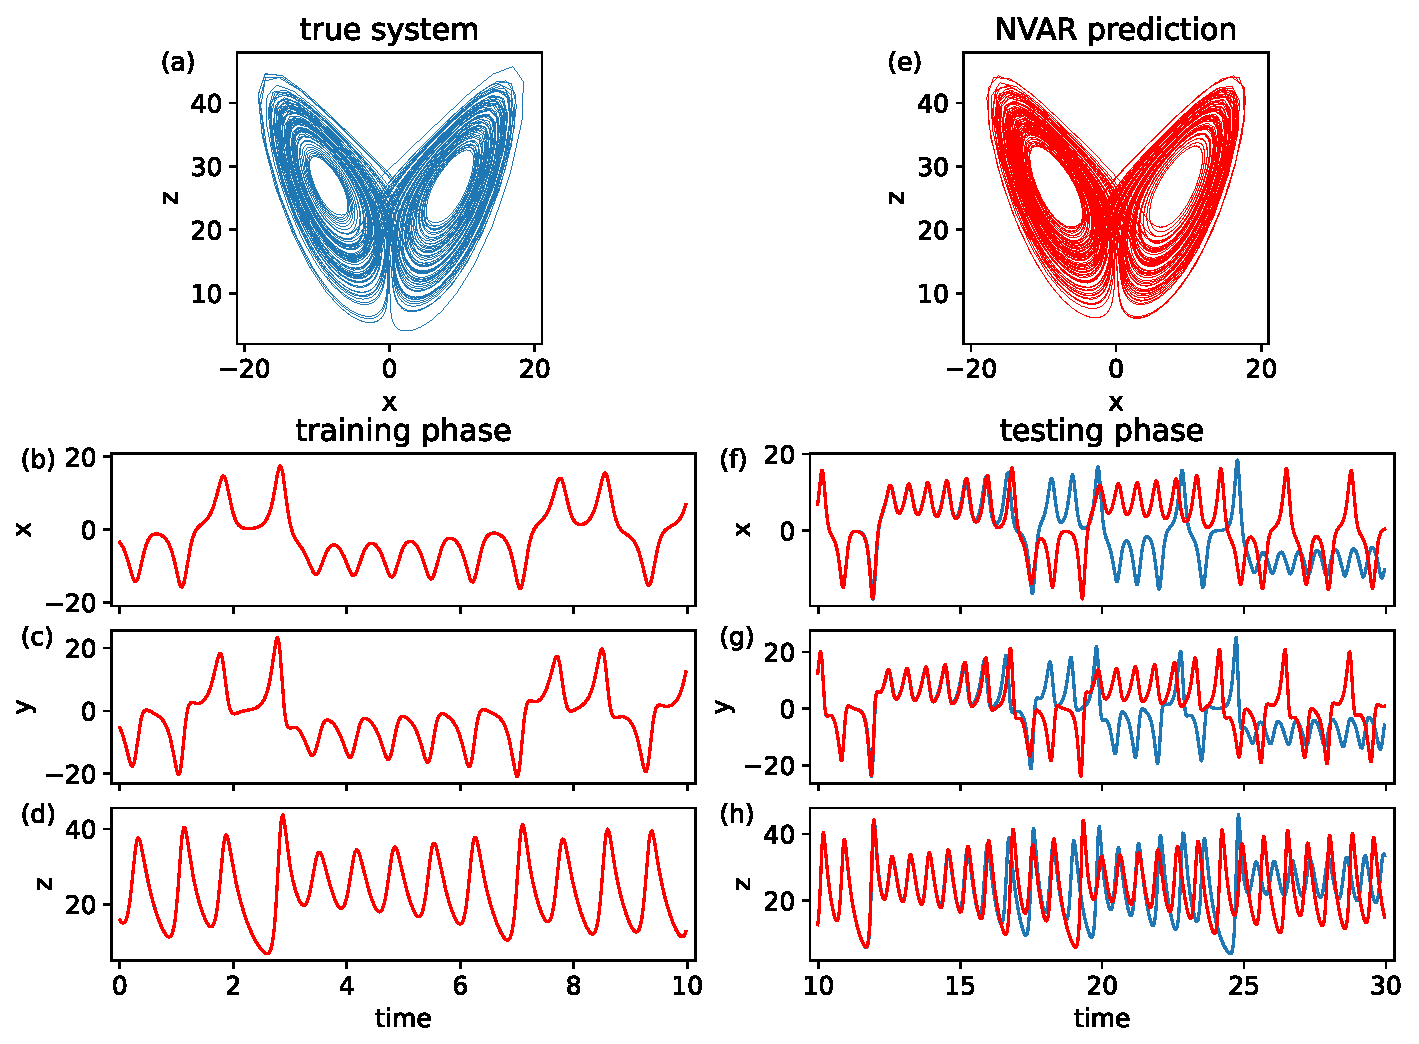
\includegraphics[width=\textwidth]{figures/nvar-predict-lorenz}
  \caption{The true Lorenz attractor (a) and NVAR predicted attractor
    (e) for a single training trial. (b)~--~(d) True Lorenz system
    (blue) during training overlaid with NVAR output (red) calculated
    after training is complete. (f)~--~(h) True (blue) and NVAR
    forecasted output (red). The NVAR shows good agreement with the
    true system as far as $6$ Lyapunov periods in to the autonomous
    forecast.}
  \label{fig:nvar-predict-lorenz}
\end{figure}

The performance of this NVAR during a single training trial is shown
in \cref{fig:nvar-predict-lorenz}. A long autonomous forecast from the
NVAR produces an attractor (e) that shows qualitative agreement with
the true Lorenz attractor (a), and produces a NRMSE over one Lyapunov
period of $4.51\pm0.85\times10^{-3}$ using $\alpha =
2.5\times10^{-6}$, about five times better than the ESNs described in
\cref{tab:lowk-lorenz-results}. This NVAR performs better than the
ESNs despite the fact that it is simpler to describe and implement,
does not require lengthy optimization, and trains at least an order of
magnitude faster. The training data used for the NVAR is also very
light: only $10$ time units, corresponding to $400$ points at this
time step, is enough to train the NVAR. During training, the NVAR's
output (b)~--~(d) matches the true signal so well it obscures it, and
during testing, the autonomous forecast (f)~--~(h) only visibly
diverges from the truth after $6$ Lyapunov exponents.

\subsection{$z$ Return Map}

The $z$ variable of the Lorenz '63 system has a functional relation
between successive local maxima. This is demonstrated visually by
finding the local maxima $z_i$ of $z$, and then plotting $z_i$ with
respect to $z_{i+1}$ \cite{lorenz1963}. This \emph{return map} neatly
summarizes the long-term behavior of the $z$ variable, and comparing
two such maps provides a quick way to qualitatively compare two
systems. This comparison has been used previously to verify that a
trained RC can replicate the Lorenz '63 dynamics~\cite{pathak2017}.

\begin{figure}
  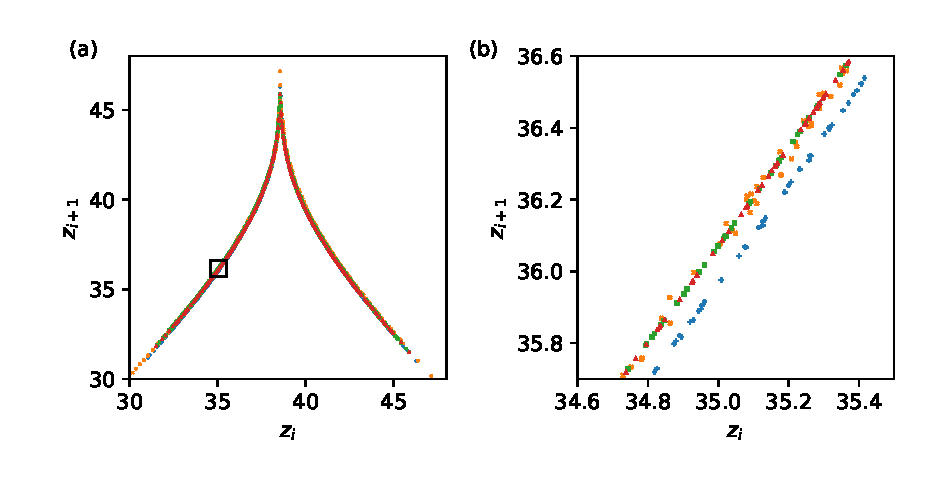
\includegraphics{figures/lorenz-rmap-tol}
  \caption{(a) The $z$ return map of the Lorenz '63 system, integrated
    using various methods. (b) Detail of the region marked in
    (a). Using a relative integration tolerance of $10^{-3}$, the
    Runge-Kutta~3(2) (blue $+$) differs from R-K~5(4) (orange
    $\times$) in both position and spread. Both methods converge after
    sharpening the tolerance to $10^{-5}$ (green square and red
    triangle, respectively).}
  \label{fig:lorenz-rmap-tol}
\end{figure}

In many ways, this comparison is similar to the visual inspection of
the reproduced attractor in \cref{fig:nvar-predict-lorenz}. However,
the return map is a simpler shape and is much more sensitive to error
than the attractor itself, even when comparing two maps by
eye. Indeed, the return map is so sensitive that it depends on the
specific integrator used to find the true Lorenz '63 solution. In
\cref{fig:lorenz-rmap-tol}, I show this return map calculated on a
Lorenz solution produced by four different integrators. All four
methods agree on a large scale, but the zoomed view in (b) reveals
their differences. Using a relative tolerance of $10^{-3}$, the
Runge-Kutta~3(2) method produces a narrow, nearly one-dimensional
return map slightly offset from the much wider return map produced by
Runge-Kutta~5(4). Both algorithms agree after sharpening the tolerance
to $10^{-5}$.  In this chapter, I use the
Runge-Kutta~3(2)~\cite{dormand1980} integrator with $10^{-3}$ relative
tolerance for both the Lorenz '63 and double-scroll systems.

The values of the maxima in the discrete-time solutions for both the
NVAR and Lorenz '63 system depend on the time step $\Delta t$ used for
integration, as the true maximum may be achieved in between the
discrete time steps. To better reproduce the true Lorenz '63 return
map, and to reduce the effect $\Delta t$ has on the NVAR return map,
I interpolate the $z$ solutions by using a degree-$4$ spline. The
local maxima are then found on this interpolated spline~\cite{dierckx1995}.

\begin{figure}
  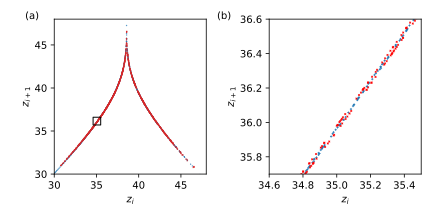
\includegraphics{figures/nvar-lorenz-rmap}
  \caption{(a) The $z$ return map of the Lorenz '63 system (blue $+$)
    overlaid with the $z$ return map of the NVAR forecast (red
    $\times$), trained for $10$ time units. The NVAR reproduces the
    long-term dynamics of the $z$ variable accurately enough at this
    scale that it is difficult to see the true return map
    underneath. (b) Detail of the region marked in (a). At this scale,
    it is possible to see that the NVAR return map is wider than the
    true Lorenz return map, although they lie on top of each
    other. This reproduction can be improved by training the NVAR for
    longer (see \cref{fig:nvar-lorenz-rmap-extra}).}
  \label{fig:nvar-lorenz-rmap}
\end{figure}

\begin{figure}
  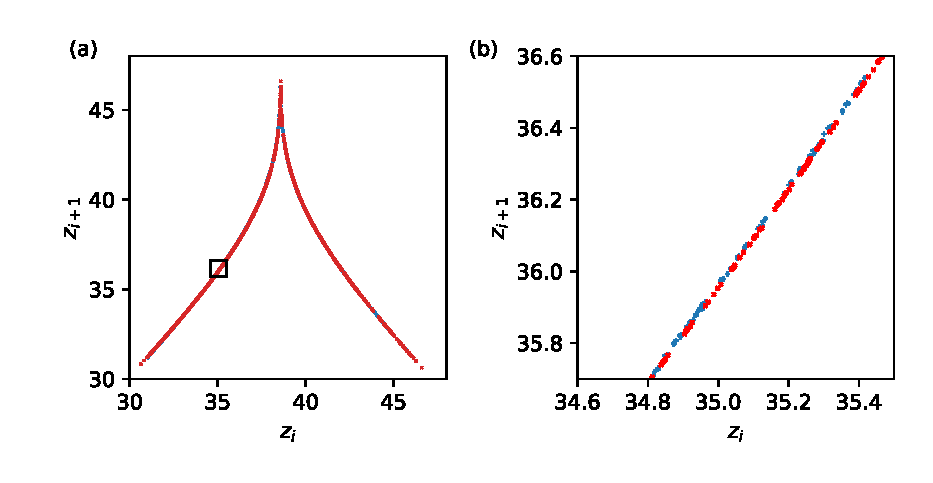
\includegraphics{figures/nvar-lorenz-rmap-extra}
  \caption{(a) The $z$ return map of the Lorenz '63 system (blue $+$)
    overlaid with the $z$ return map of the NVAR forecast (red
    $\times$), trained for $20$ time units. (b) Detail of the
    region marked in (a). With more training time, the NVAR return map
    is narrower and more accurately reproduces the Lorenz return
    map.}
  \label{fig:nvar-lorenz-rmap-extra}
\end{figure}

\Cref{fig:nvar-lorenz-rmap} shows the return maps for both the true
Lorenz system and the NVAR. Qualitatively, there is good agreement
between the two. The NVAR return map almost completely obscures the
true Lorenz return map in (a). Upon close inspection in (b), I see
that the NVAR return map has a width that is wider than that of the
true return map. This can be improved by extending the training time
of the NVAR. The difference between the two return maps is already
small even when the NVAR is trained for only $10$ time units; when
training for $20$ time units, as in \cref{fig:nvar-lorenz-rmap-extra},
the NVAR's predicted return map narrows and lies on top of the true
return map.

As with the attractor comparison, a quantitative measure of return map
similarity would be a strong candidate for replacing the flawed NRMSE
measure.

\subsection{Fixed Points}

For a more quantitative measure of how well the NVAR learns the
dynamics of the Lorenz system, I calculate the fixed points of the
trained NVAR and then find their distance to the true Lorenz steady
states. This comparison has also been used for reservoir computers~\cite{krishnagopal2019}. For simplicity and consistency, in this dissertation I will
refer to both the discrete-time fixed points of the NVAR and the
continuous-time steady states of Lorenz and other systems as ``fixed
points''.

By setting the derivatives in \cref{eq:lorenz} to zero, I
find three fixed points of the Lorenz system located at
\begin{align}
  [x, y, z] &= [0, 0, 0], \\
            &= [\pm \sqrt{\beta(\rho - 1)}, \pm \sqrt{\beta(\rho - 1)}, (\rho - 1)].
\end{align}

To find the fixed points of the NVAR system, I perform a trial
single-step forecast with a constant past history, and use the Powell hybrid method
root-finding algorithm~\cite{more1980,powell1970} to find the specific values of past history
that result in an unchanged forecast. This root-finding algorithm is
used three times, using the three true Lorenz fixed points as initial
guesses.

To allow easy comparison of the accuracy of these fixed points with
other systems, I calculate the distance between this fixed points in
a uniformly scaled space where the Lorenz63 system has unit
variance. For this trained NVAR, the distance from the zero fixed point
is $1.2\pm1.4\times10^{-3}$, and the distances between the predicted
and true positive and negative fixed points are
$11.6\pm3.0\times10^{-4}$ and $7.4\pm1.5\times10^{-4}$, respectively.
% FIXME compare (I can't find any quantitative results!)

The NVAR shows good agreement on the zero fixed point, as the variance
caused by different training windows overlaps with the true
location. The other two fixed points are consistently offset from the
truth. However, in all three cases, the fixed points lie within
approximately $0.1\%$ of the true location, despite the fact that the
training data does not include any of these points.

\subsection{Output Weights}

The particular choice of nonlinearity $\bm{g}_\text{n}$ for this task
completely includes all terms in the vector field of the Lorenz
system in \cref{eq:lorenz}. That is, the Lorenz system is described by
a polynomial of degree $2$, and the choice of $\bm{g}_\text{n}$ allows
the NVAR to describe \emph{any} polynomial of degree $2$. This raises
a legitimate question: is the NVAR simply performing so well because
it was equipped ahead of time with the perfect tools?

The answer in a general context is no. Just as a finite truncation of an infinite Taylor series can
approximate non-polynomial functions arbitrarily well, a continuous
nonlinear dynamical system can be approximated arbitrarily well by a
finite Volterra series~\cite{franz2006}, and NVARs with polynomial
outputs are finite Volterra series with very simple kernels. From this
fact, I expect NVARs with quadratic nonlinearity to be able to
approximate even non-polynomial systems, and so it is not surprising
that it can also approximate quadratic polynomial systems.

\begin{figure}
  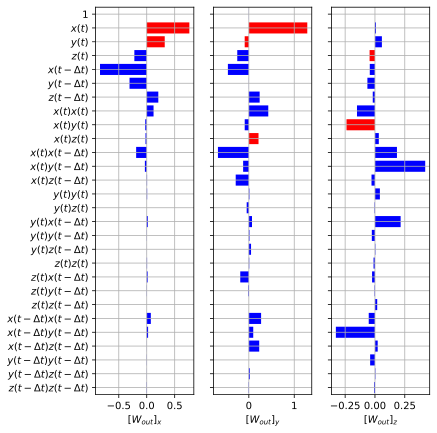
\includegraphics[width=\textwidth]{figures/nvar-predict-lorenz-wout}
  \caption{Weights in the matrix $W_\text{out}$ for the NVAR trained
    for Lorenz system forecasting. Terms that appear directly in the
    Lorenz system (\cref{eq:lorenz}) are in dashed red. There does not appear
    to be any correlation between a large weight in the NVAR output,
    and presence in the Lorenz equations.}
  \label{fig:nvar-predict-lorenz-wout}
\end{figure}

Another way to allay these concerns is to look at other non-polynomial
systems, as in the next few sections. However, even with the Lorenz
system, I see that this is not the case by inspecting the trained
weight matrix $W_\text{out}$ in
\cref{fig:nvar-predict-lorenz-wout}. The terms on the right hand side
of the Lorenz system (marked in red) are present with non-zero weights
in the output matrix, but there are also significant contributions
from other terms, and there does not appear to be a preference for the
NVAR to rely on Lorenz terms only.

From this I derive an interpretation: a trained NVAR is finding the
best possible one-step-ahead integrator it can find, given the example
input and the available terms in $\bm{g}_\text{n}$. When the time step
is large enough, a strictly linear prediction becomes more and more
inaccurate, and so the NVAR relies on the nonlinear and time-delayed
terms to make up the difference.

\section{Forecasting the Double-Scroll Circuit}

For this task, I use an NVAR in forecasting mode to use all
three state variables $V_1$, $V_2$, and $I$ of the double-scroll
circuit described by \cref{eq:dscroll}. I use the same tap
delays $\tau_0 = 0$, $\tau_1 = 1$ as the Lorenz case, but I modify
the choice of nonlinearity.

Unlike the Lorenz system, the double-scroll circuit cannot be
described by a polynomial of degree $2$. Indeed, the double-scroll
equations are odd, and have full inversion symmetry. On top of this,
the double-scroll attractor includes this symmetry; it is identical to
its symmetric partner. As discussed in \cref{sec:nvar-infer-weights},
this drives the contribution of any even terms in $\bm{g}_\text{n}$ to
zero in the trained weight matrix $W_\text{out}$. In light of this, I
use a nonlinear function that includes all linear terms of the tap
vector $\bm{v}$ as well as all terms with degree $3$, but includes no
even terms. That is,
\begin{equation}
  \bm{g}_\text{n}(\bm{v}) = \bm{v} \oplus \ceil{\bm{v} \otimes \bm{v} \otimes \bm{v}}.
\end{equation}
With $q = 2$ taps and $d = 3$ input dimensions, the output of
$\bm{g}_\text{n}$ has $6 + 56 = 62$ components, and so $W_\text{out}$
has dimension $3 \times 62$.

The Lyapunov time of the double-scroll circuit is roughly $10$ times
longer than that of the Lorenz system. To ensure a fair comparison, I
extend the training time of the NVAR from $10$ to $100$ units to keep
the number of Lyapunov times covered by the training similar for both
cases. I also set $\Delta t = 0.25$, to ensure that both the Lorenz
and double-scroll cases use $400$ data points during training.

\begin{figure}
  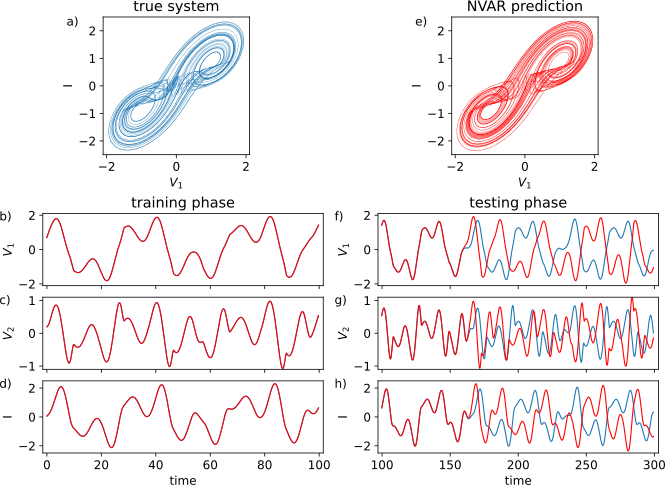
\includegraphics[width=\textwidth]{figures/nvar-predict-dscroll}
  \caption{The true double-scroll attractor (a) and NVAR predicted
    attractor (e) for a single training trial. (b)~--~(d) True
    double-scroll system (blue) during training overlaid with NVAR
    output (red) calculated after training is complete. (f)~--~(h)
    True (blue) and NVAR forecasted output (red). Here, the NVAR
    shows good agreement with the true system as far as $6$ Lyapunov
    periods.}
  \label{fig:nvar-predict-dscroll}
\end{figure}

Other than these modifications, the method for using the NVAR to
forecast the dynamics of this system proceeds exactly as for the Lorenz
system, training the NVAR on $10$ different examples of the
double-scroll circuit and then evaluating the NRMSE for one Lyapunov
period each. The performance of this NVAR during a single training
trial is shown in \cref{fig:nvar-predict-dscroll}.

Once again, a long autonomous forecast (e) shows the NVAR can
reproduce the shape of the double-scroll attractor (a), and over one
Lyapunov period has an NRMSE of $2.15\pm0.63\times10^{-2}$ using
$\alpha = 1.0\times10^{-3}$, about $1.5\times$ better than the ESNs
described in \cref{tab:lowk-resultsplus}. During training (b)~--~(d)
the NVAR matches the system so well the true signal cannot be seen
underneath, and once autonomous forecasting begins in (f)~--~(h), the
NVAR's prediction lies on top of the true system for $6$ Lyapunov
periods.

\subsection{Fixed Points}

Again, I look for the fixed points of this trained NVAR and find
their distance to the true fixed points of the double-scroll circuit,
in a space uniformly scaled so that the double-scroll circuit has unit
variance. Setting the derivatives in \cref{eq:dscroll} to $0$
and solving yields the transcendental equation
\begin{equation}
  0 = \frac{V_1}{R_2}(R_1 - R_2 - R_4) + 2 R_1 I_r \sinh\left(\alpha V_1 \left(1 - \frac{R_4}{R_1}\right)\right).
\end{equation}
For the parameters I use, this yields three solutions for $V_1$. If
$V_1^+$ is the positive solution, this corresponds to three fixed points
at
\begin{align}
  [V_1, V_2, I] &= [0, 0, 0], \\
                &= [V_1^+, \pm V_1^+ R_4 / R_1, \pm V_1^+ / R_1].
\end{align}

Since my choice of $\bm{g}_\text{n}$ has only odd polynomial powers
and no constant term, it is symmetric about the origin and predicts
the zero fixed point exactly. The distance from the true positive
fixed point is $2.7\pm0.3\times10^{-3}$. Due to the inversion
symmetry, the negative fixed point is precisely the same
distance. Although the variance from repeated trials does not overlap
the true fixed points, they do lie within $0.3\%$ of the truth.

This NVAR performs well at short-term forecasting and fixed point
prediction, despite not having access to the infinite number of
polynomial terms in the expansion of the double-scroll equations. This
demonstrates a possible practical approach to NVAR design: keep adding
delay taps and higher polynomial terms to the nonlinear function
$\bm{g}_\text{n}$ until performance is acceptable. However, for NVARs
that require many taps or operate on high-dimensional inputs, this
very quickly leads to an explosion in the number of weights trained in
$W_\text{out}$, and consequently a huge increase in training time. In
the next section, I explore how careful use of tap spacing can
keep the number of taps required low.

\section{Forecasting Mackey-Glass}\label{sec:nvar-mackey-glass}

For this task, I again use an NVAR in forecasting mode, this time
using the single Mackey-Glass state variable $u$ in
\cref{eq:mackey-glass} as input, with $\Delta t = 0.2$. I use the
\texttt{jitcdde} Python package~\cite{ansmann2018} to integrate this
time-delay differential equation. For this system, using two adjacent
taps for the NVAR as in the previous examples is not enough, as the
Mackey-Glass system behavior depends strongly on both the value of
$u(t)$ as well as $u(t - 17)$. One way to access this value in the
NVAR is to add taps at every time step until they reach $t = 17$,
resulting in $85$ total taps. Even with only a quadratic output, this
requires training a $W_\text{out}$ with dimension $1 \times
3741$. This cost can be avoided by increasing the time step $\Delta
t$, thus reducing the total number of taps, but this solution comes
with the cost of a much more granular prediction. Granularity may not
be a problem, as up to a point, as the NVAR's predictions can be
interpolated to fill in the gaps. However, using a coarser $\Delta t$
also changes the behavior of the NVAR, and for this task results in
poor performance.

Another way to access the value at $u(t-17)$ is to use sparse
taps. Here, I use three clusters of two adjacent taps: one cluster at
$\tau_0 = 0$ and $\tau_1 = 1$, one cluster at $\tau_2 = \floor{17 / 2
  \Delta t}$ and $\tau_3 = \tau_2 + 1$, and one cluster at $\tau_4 =
\floor{17 / \Delta t}$ and $\tau_5 = \tau_4 + 1$. Here, $\floor{a}$ refers to the integer floor of $a$. This gives the NVAR
access to information at $u(t - 17)$ as well the midpoint $u(t -
17/2)$. I find that adding the tap cluster at the midpoint improves performance
by a factor of $3$, and increases the number of features available to
$W_\text{out}$ to be comparable to the other tasks in this chapter.

The Mackey-Glass system exhibits full inversion symmetry. However,
unlike the double-scroll circuit, the Mackey-Glass system has two
distinct attractors that do not overlap. Any solution on the positive
attractor will remain positive, and never cross over zero to the
negative attractor. Since I am only training the NVAR on a positive
solution to Mackey-Glass, I include even terms in $\bm{g}_\text{n}$. In
fact, I find that including these even terms improves NRMSE
performance. In \cref{sec:nvar-mg-weights}, I demonstrate that the trained NVAR is assigning these terms non-zero weights.

Therefore, I use a nonlinear function
$\bm{g}_\text{n}$ that includes the constant, linear, quadratic, and
cubic terms constructed from the tap vector $\bm{v}$,
\begin{equation}
  \bm{g}_\text{n}(\bm{v}) = 1 \oplus \bm{v} \oplus \ceil{\bm{v} \otimes \bm{v}} \oplus \ceil{\bm{v} \otimes \bm{v} \otimes \bm{v}}.
\end{equation}
With $q = 6$ taps and $d = 1$ input dimension, the output of $\bm{g}_\text{n}$
has $1 + 6 + 21 + 56 = 84$ components, and so $W_\text{out}$ has
dimension $1 \times 84$.

The Lyapunov time of the Mackey-Glass system is roughly $100$ times
longer than that of the Lorenz system. However, I find that a
relatively fine step size $\Delta t = 0.2$ is required for the NVAR to
learn the system, corresponding to $500$ points per Lyapunov period. I train this NVAR for $1000$ time units,
corresponding to $5000$ data points total. Though this is many more
discrete data points, it covers about $10$ Lyapunov times, comparable
to the training time used for the other systems.

This NVAR is much more data hungry than the previous examples,
requiring more training data to produce an acceptable result. This may
be due to the wide tap spacing: values at $u(t - 17)$ are less
correlated to $u(t)$, while $u(t - \Delta t)$ is more correlated, and
so the NVAR needs more data to see every relevant combination of
values at the taps.

\begin{figure}
  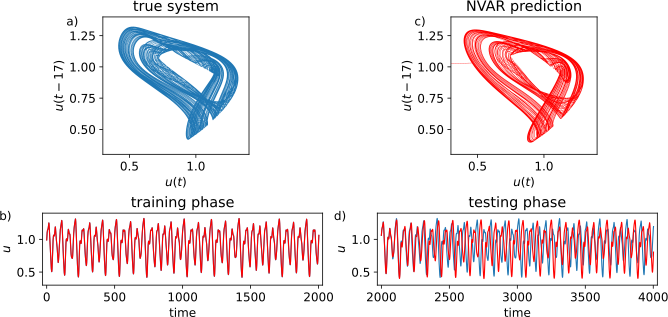
\includegraphics[width=\textwidth]{figures/nvar-predict-mackey-glass}
  \caption{The true Mackey-Glass attractor (a) and NVAR predicted
    attractor (c) for a single training trial. (b) True Mackey-Glass
    system during training overlaid with NVAR output (red) calculated
    after training is complete. (d) True (blue) and NVAR forecasted
    output (red). Here, the NVAR shows good agreement with the true
    system as far as $2$ Lyapunov periods.}
  \label{fig:nvar-predict-mackey-glass}
\end{figure}

Other than these modifications, the methodology for training and
evaluating the NVAR is exactly as for the other two systems. The
performance of this NVAR during a single training trial is shown in
\cref{fig:nvar-predict-mackey-glass}. Over one Lyapunov period, this
NVAR has a NRMSE of $5.77\pm0.42\times10^{-2}$ with $\alpha =
9\times10^{-3}$.

The long autonomous forecast (c) of the NVAR shares important features
with the true attractor (a), most notably the gap between the
bands. However, it does not get some fine details correct, notably the
shape of the heel in the upper-left corner and the overlapping bands
in the middle. This is reflected in the higher NRMSE than the other
tasks. However, as before the NVAR prediction completely obscures the
true system signal during training (b), and once autonomous
forecasting (d) begins the NVAR forecast covers the true system for $2$
Lyapunov periods.

The shape of this heel can be better reproduced by including
higher-order terms in the nonlinear function
$\bm{g}_\text{out}$. However, it is not possible to do this with
monomial terms as I have been doing without dramatically increasing
the training time of $W_\text{out}$. Adding a fourth-order term to $\bm{g}_\text{out}$ increases the number of weights in $W_\text{out}$ by a factor of $3$. This problem becomes even worse on input systems with a dimension higher than $d = 1$.

It may be possible to instead add
nonlinear terms to $\bm{g}_\text{out}$ with an infinite power series,
such as $e^{v_iv_j}$ or $\sinh{v_i}\cosh{v_j}$. This would provide
access to high-order nonlinearity without a corresponding large increase in training
time. This is one important avenue for future research, and this
Mackey-Glass forecasting example demonstrates that cubic terms are not
completely sufficient for accurate forecasts. Nonetheless, the cubic
NVAR used here shows promising performance from a simple model.

\subsection{Fixed Points}

Setting the derivative in \cref{eq:mackey-glass} to $0$ and assuming a
constant past yields three fixed points, located at
\begin{align}
  u &= 0, \\
  u &= \pm \left(\frac{\beta}{\gamma} - 1\right)^{1/n}.
\end{align}
I use these as initial guesses to find the fixed points of the trained NVAR, in a space uniformly scaled so that Mackey-Glass has unit variance.

The distance to the true positive fixed point is
$2.25\pm0.03\times10^{-3}$. The variance from repeated trials does not
overlap the true fixed point, however, it does lie within $0.3\%$ of
the truth.

The NVAR completely fails to predict the $0$ fixed point and the
negative fixed point. This is a consequence of my choice not to
respect the known symmetries of the Mackey-Glass system in favor of
more accurate prediction on the positive attractor. If accuracy on the
non-positive fixed points is desired, the NVAR can be either modified
to respect that symmetry ahead of time, or trained on data from both
the positive and negative attractors.

\subsection{Output Weights}\label{sec:nvar-mg-weights}

The output weights for this task are in
\cref{fig:nvar-predict-mackey-glass-wout}. As expected from the
failure to predict the non-positive fixed points, the NVAR
assigns non-zero weights to those terms (in red) that break the
total inversion symmetry. As the training input does not include any
data from the negative Mackey-Glass attractor, the NVAR has no cause
to learn this symmetry and instead utilizes these terms to improve
forecasting accuracy on the positive attractor. That the NVAR assigns
non-zero weights to these terms, and that the resulting NVAR performs
better than one constructed without these terms, justifies my
inclusion of the even terms in this NVAR and demonstrates that an NVAR
can use symmetry-breaking terms productively as long as it is only
used for forecasting in an area of the underlying system that does not
contain that symmetry.

\begin{sidewaysfigure}
  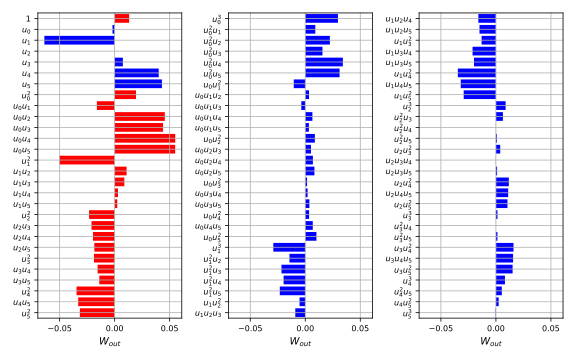
\includegraphics[width=\textwidth]{figures/nvar-predict-mackey-glass-wout}
  \caption{Weights in the matrix $W_\text{out}$ for the NVAR trained
    for Mackey-Glass system forecasting. Terms that break the
    inversion symmetry are in dashed red. In labels, $u_i$ is shorthand for $u(t - \tau_i \Delta t)$. As the training signal does not
    reflect the inversion symmetry, the red terms are not trained to
    near zero as they are in \cref{fig:nvar-infer-lorenz-wout}.}
  \label{fig:nvar-predict-mackey-glass-wout}
\end{sidewaysfigure}

\section{Conclusion}

In this chapter, I demonstrate the NVAR approach on two classic
RC problems: state inference and system forecasting.
These results are summarized in \cref{tab:nvar-results}.
I show that
NVARs can solve these problems as well, or in some cases better, than
the RC approach, despite the simplicity of the NVAR method. At the
same time, I resolve the remaining questions raised in
\cref{ch:nvar}: NVARs remain useful even with only a handful of
time-delay taps, and a simple extension of the nonlinear function
$\bm{g}_\text{n}$ to include higher-order monomial terms is sufficient
in many cases.

\begin{table}
  \caption{Summary of results in this chapter: the dimension of
    $W_\text{out}$, the ridge parameter $\alpha$, the NRMSE
    ($\epsilon$ for inference, $\tilde{\epsilon}$ for forecasting),
    and the normalized distance from true fixed points to predicted
    fixed points.}
  \begin{tabularx}{\linewidth}{llreff}
    \multicolumn{2}{l}{Task} & \multicolumn{1}{c}{$W_\text{out}$} & \multicolumn{1}{c}{$\alpha$} & \multicolumn{1}{c}{$\epsilon$ / $\tilde{\epsilon}$} & \multicolumn{1}{c}{Fixed Points} \\
    \hline
    \rule{0pt}{4ex}
    Lorenz '63 & Inference & $1 \times 45$ & 5.0\times10^{-2} & 1.75\pm0.3\times10^{-2} & \multicolumn{1}{c}{--} \\
    \rule{0pt}{4ex}
    Lorenz '63 & Forecasting & $3 \times 28$ & 2.5\times10^{-6} & 4.51\pm0.9\times10^{-3} & 1.2\pm1.4\times10^{-3} \\
    &&&&& 11.6\pm3.0\times10^{-4} \\
    &&&&& 7.4\pm1.5\times10^{-4} \\
    \rule{0pt}{4ex}
    Double-Scroll & Forecasting & $3 \times 62$ & 1.0\times10^{-3} & 2.15\pm0.6\times10^{-2} & 2.7\pm0.3\times10^{-3} \\
    \rule{0pt}{4ex}
    Mackey-Glass & Forecasting & $1 \times 84$ & 9.0\times10^{-3} & 5.77\pm0.4\times10^{-2} & 2.25\pm0.03\times10^{-3} \\
  \end{tabularx}
  \label{tab:nvar-results}
\end{table}

The Mackey-Glass forecasting task sits at the very edge of this simple
technique. It shows that a low number of time-delay taps is
enough even in systems with long, built-in time delays, as long as the taps are chosen carefully. However,
it also demonstrates that a cubic nonlinearity is not enough to
reproduce the precise shape of the Mackey-Glass attractor. To move
forward with the NVAR technique, the nonlinear function
$\bm{g}_\text{n}$ needs to include higher-order terms, and it
needs to do so without the exponential increase in training time
associated with adding more monomial terms to the output.

The Mackey-Glass system also demonstrates that symmetry matching is
not necessary or even desired in all cases when using an NVAR, if the
signal the NVAR is trained on never encounters that symmetry. In that
case, the NVAR will utilize terms that break the symmetry of the
underlying system in order to improve forecasting accuracy within the
volume of phase space that the training signal lies inside. This comes
with a trade-off: prediction outside this volume of phase space, such
as predicted fixed points, fails.

Even with the unresolved questions, I find the NVAR method is very
simple to implement and performs well. Due to its simplicity, I
recommend attempting to use an NVAR first in all cases where an RC is
considered.

\chapter{Conclusion}\label{ch:conclusion}

In this thesis, I challenge common RC design rules, and
demonstrate increasingly simple RCs that break these rules and still
perform well.

In \cref{ch:low-connectivity}, I demonstrate ESN-based RCs with five
classes of simple internal connectivity that all perform well on the
system forecasting task. Despite the fact that recurrence is a common
requirement in ESN design, two of these classes of connectivity have
\emph{no recurrence}, but continue to perform. A network with only a
single internal cycle, or no cycles at all, can perform as well as a
network with many recurrent cycles. These simpler reservoir structures
may benefit hardware-based RCs, where every internal connection has an
associated cost.

This work reveals some new lines of possible future
research. Primarily, the $\tilde{\epsilon}$ metric is a more valuable
measure than $\epsilon_1$ of how well the ESN reproduces the climate
of the system, but ultimately still fails to measure attractor
similarity directly. The development of such a metric would be very
important to the field, as it begins to consider how well an RC
reproduces climate in addition to short-term forecasting.

One of the simple connectivity classes I explore is a simple line
network. The fact that this line network can perform as well as a
full-connectivity network indicates that perhaps the reservoir's role
is to produce a variety of time delays for the RC output layer to draw
on. In \cref{ch:nvar}, I summarize the NVAR method, which parallels
the RC method but instead takes time-delay taps of the input directly
rather than relying on a reservoir. I also sketch a new proof in the
field of reservoir computing that shows a certain type of
output-non-linear ESN is equivalent to an infinite-tap NVAR.

In \cref{ch:nvar-application} I build on this proof with my
collaborators to implement NVARs that solve the traditional RC tasks
of system state inference and system forecasting. I show
that the NVAR can solve these tasks with only a few, finite taps, and
that the specific non-linearity used in the proof can be modified an
extended in obvious ways to expand the number of problems it can
solve. This opens the door to an entire expanding tree of interesting
research. Now any task previously solved in an RC context can be
attempted in an NVAR context, and the success or failure of the NVAR
at solving a given problem will contribute meaningfully to both the
NVAR and RC fields.

Applying the NVAR approach to Mackey-Glass system forecasting reveals
possibly the most important avenue for future research. Cubic terms
are not sufficient for all problems, but adding higher-order monomials
directly to the NVAR leads to an exponential explosion in training
time. Future research will need to resolve this by including these
higher-order terms without exhaustively including all monomials, and
may possibly make use of non-linear functions with infinite power
series.

The NVAR is a reservoir computer pruned down to its most essential
components, and now that I know it is possible build a high-performance reservoir computer
without a reservoir \emph{at all}, I am excited to see what new
directions the RC field moves towards.


\backmatter
%\nocite{*}
\bibliography{thesis}

\appendix
\chapter{Example Systems}\label{ch:systems}

Reservoir computers are most useful as tools for answering questions
about dynamic systems, such as state inference and
forecasting. Throughout this thesis, I use many small chaotic systems
for example RC tasks. For reference, they are included here.

\section{Lorenz '63}\label{sec:lorenz}

\begin{figure}
  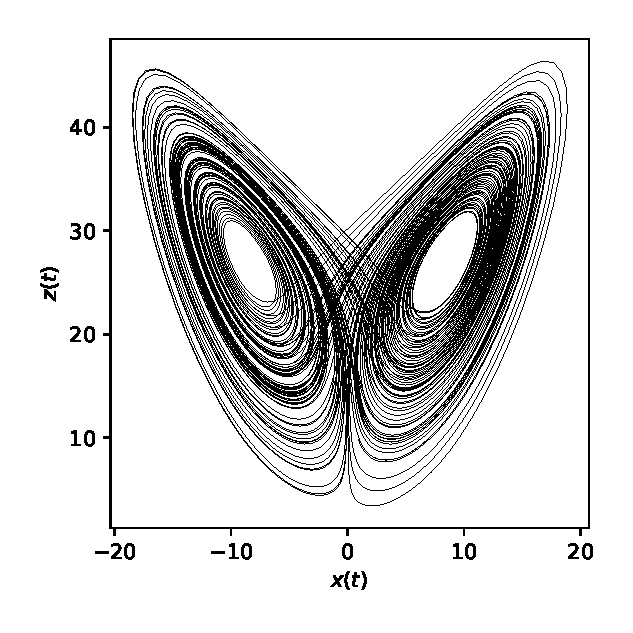
\includegraphics[width=0.6\textwidth]{figures/lorenz}
  \caption{The true Lorenz attractor in the $x$/$z$ plane, produced by integrating \cref{eq:lorenz}.}%
  \label{fig:lorenz}
\end{figure}

The Lorenz '63 chaotic system is described by
\begin{equation}
  \begin{aligned}
    \dot{x} &= 10 \left(y - x\right), \\
    \dot{y} &= x \left(28 - z\right) - y, \\
    \dot{z} &= x\,y - \frac{8}{3} z,
  \end{aligned}
  \label{eq:lorenz}
\end{equation}
with standard parameters.\cite{lorenz1963} The attractor of this
system can be visualized easily in two dimensions by projecting the
three-dimensional trajectory of the system onto a plane. I show the
attractor in the $x$/$z$ plane in \cref{fig:lorenz}.

\section{R{\"{o}}ssler}\label{sec:rossler}

\begin{figure}
  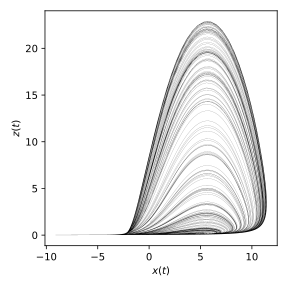
\includegraphics[width=0.6\textwidth]{figures/rossler}
  \caption{The true R{\"{o}}ssler attractor in the $x$/$z$ plane, produced by integrating \cref{eq:rossler}.}%
  \label{fig:rossler}
\end{figure}

The R{\"{o}}ssler system is described by
\begin{equation}
  \begin{aligned}
    \dot{x} &= - y - z, \\
    \dot{y} &= x + a y, \\
    \dot{z} &= b + z (x - c),
  \end{aligned}
  \label{eq:rossler}
\end{equation}
with standard parameters $a = 0.2$, $b = 0.2$, $c =
5.7$.\cite{rossler1976} The attractor of this system is visualized in
\cref{fig:rossler}.

The $z$ component of this system mostly stays near zero, with rare
positive spikes. This makes prediction with an RC difficult. To make
this component of the system more suitable for RC prediction, I use
$\log z$ instead for both RC input and prediction output.

\section{Double-Scroll}\label{sec:dscroll}

\begin{figure}
  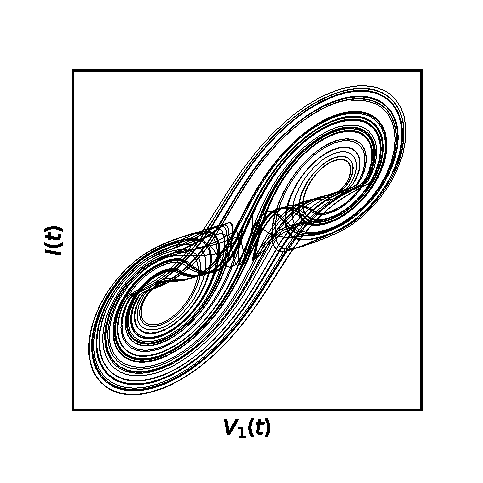
\includegraphics[width=0.6\textwidth]{figures/dscroll}
  \caption{The true double-scroll circuit attractor in the $V_1$/$I$ plane, produced by integrating \cref{eq:dscroll}.}%
  \label{fig:dscroll}
\end{figure}

The double-scroll chaotic circuit is described by the dimensionless equations
\begin{equation}
 \begin{aligned}
   \dot{V_1} &= \frac{V_1}{R_1} - \frac{V_1 - V_2}{R_2} - 2 I_r \sinh\left(\alpha(V_1 - V_2)\right), \\
   \dot{V_2} &= \frac{V_1 - V_2}{R_2} + 2 I_r \sinh\left(\alpha(V_1 - V_2)\right) - I, \\
   \dot{I} &= V_2 - R_4 I,
 \end{aligned}
 \label{eq:dscroll}
\end{equation}
with parameters $R_1 = 1.2$, $R_2 = 3.44$, $R_4 = 0.193$, $I_r = 2.25
\times 10^{-5}$, and $\alpha = 11.6$.\cite{gauthier1996} The attractor
of this system is visualized in \cref{fig:dscroll}.

\section{Mackey-Glass}\label{sec:mackey-glass}

\begin{figure}
  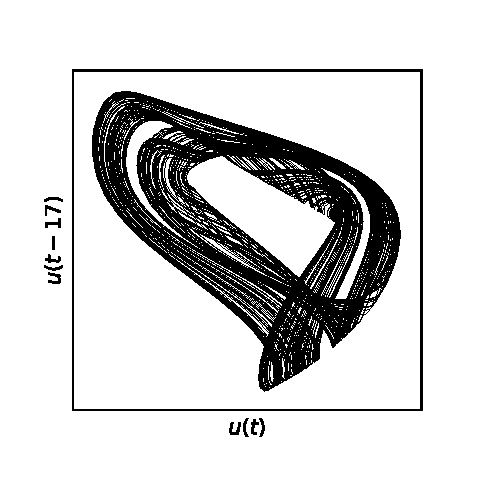
\includegraphics[width=0.6\textwidth]{figures/mackey-glass}
  \caption{The true Mackey-Glass attractor represented as a time delay embedding using $\tau$ as the delay, produced by integrating \cref{eq:mackey-glass}.}%
  \label{fig:mackey-glass}
\end{figure}

The Mackey-Glass system is described by the time-delay differential equation
\begin{equation}
  \dot{u}(t) = \beta \frac{u(t - \tau)}{1 + u(t - \tau)^n} - \gamma u(t),
  \label{eq:mackey-glass}
\end{equation}
with standard parameters $\beta = 0.2$, $\gamma = 0.1$, $\tau = 17$,
$n = 10$.\cite{mackey1977} The attractor of this system is most
commonly visualized as a time-delay embedding of the trajectory, using
$\tau$ as the delay parameter, as depicted in \cref{fig:mackey-glass}.


\end{document}
